\chapter{Comparaison des affichages}

	\section{Avec labels}
	
\paragraph{}Nous allons à présent comparer le rendu visuel de nos différents générateurs ainsi que de GraphViz qui est de nos jours l'outil le plus utilisé.
	
\paragraph{GraphViz}

\begin{figure}[h!]
\begin{center}
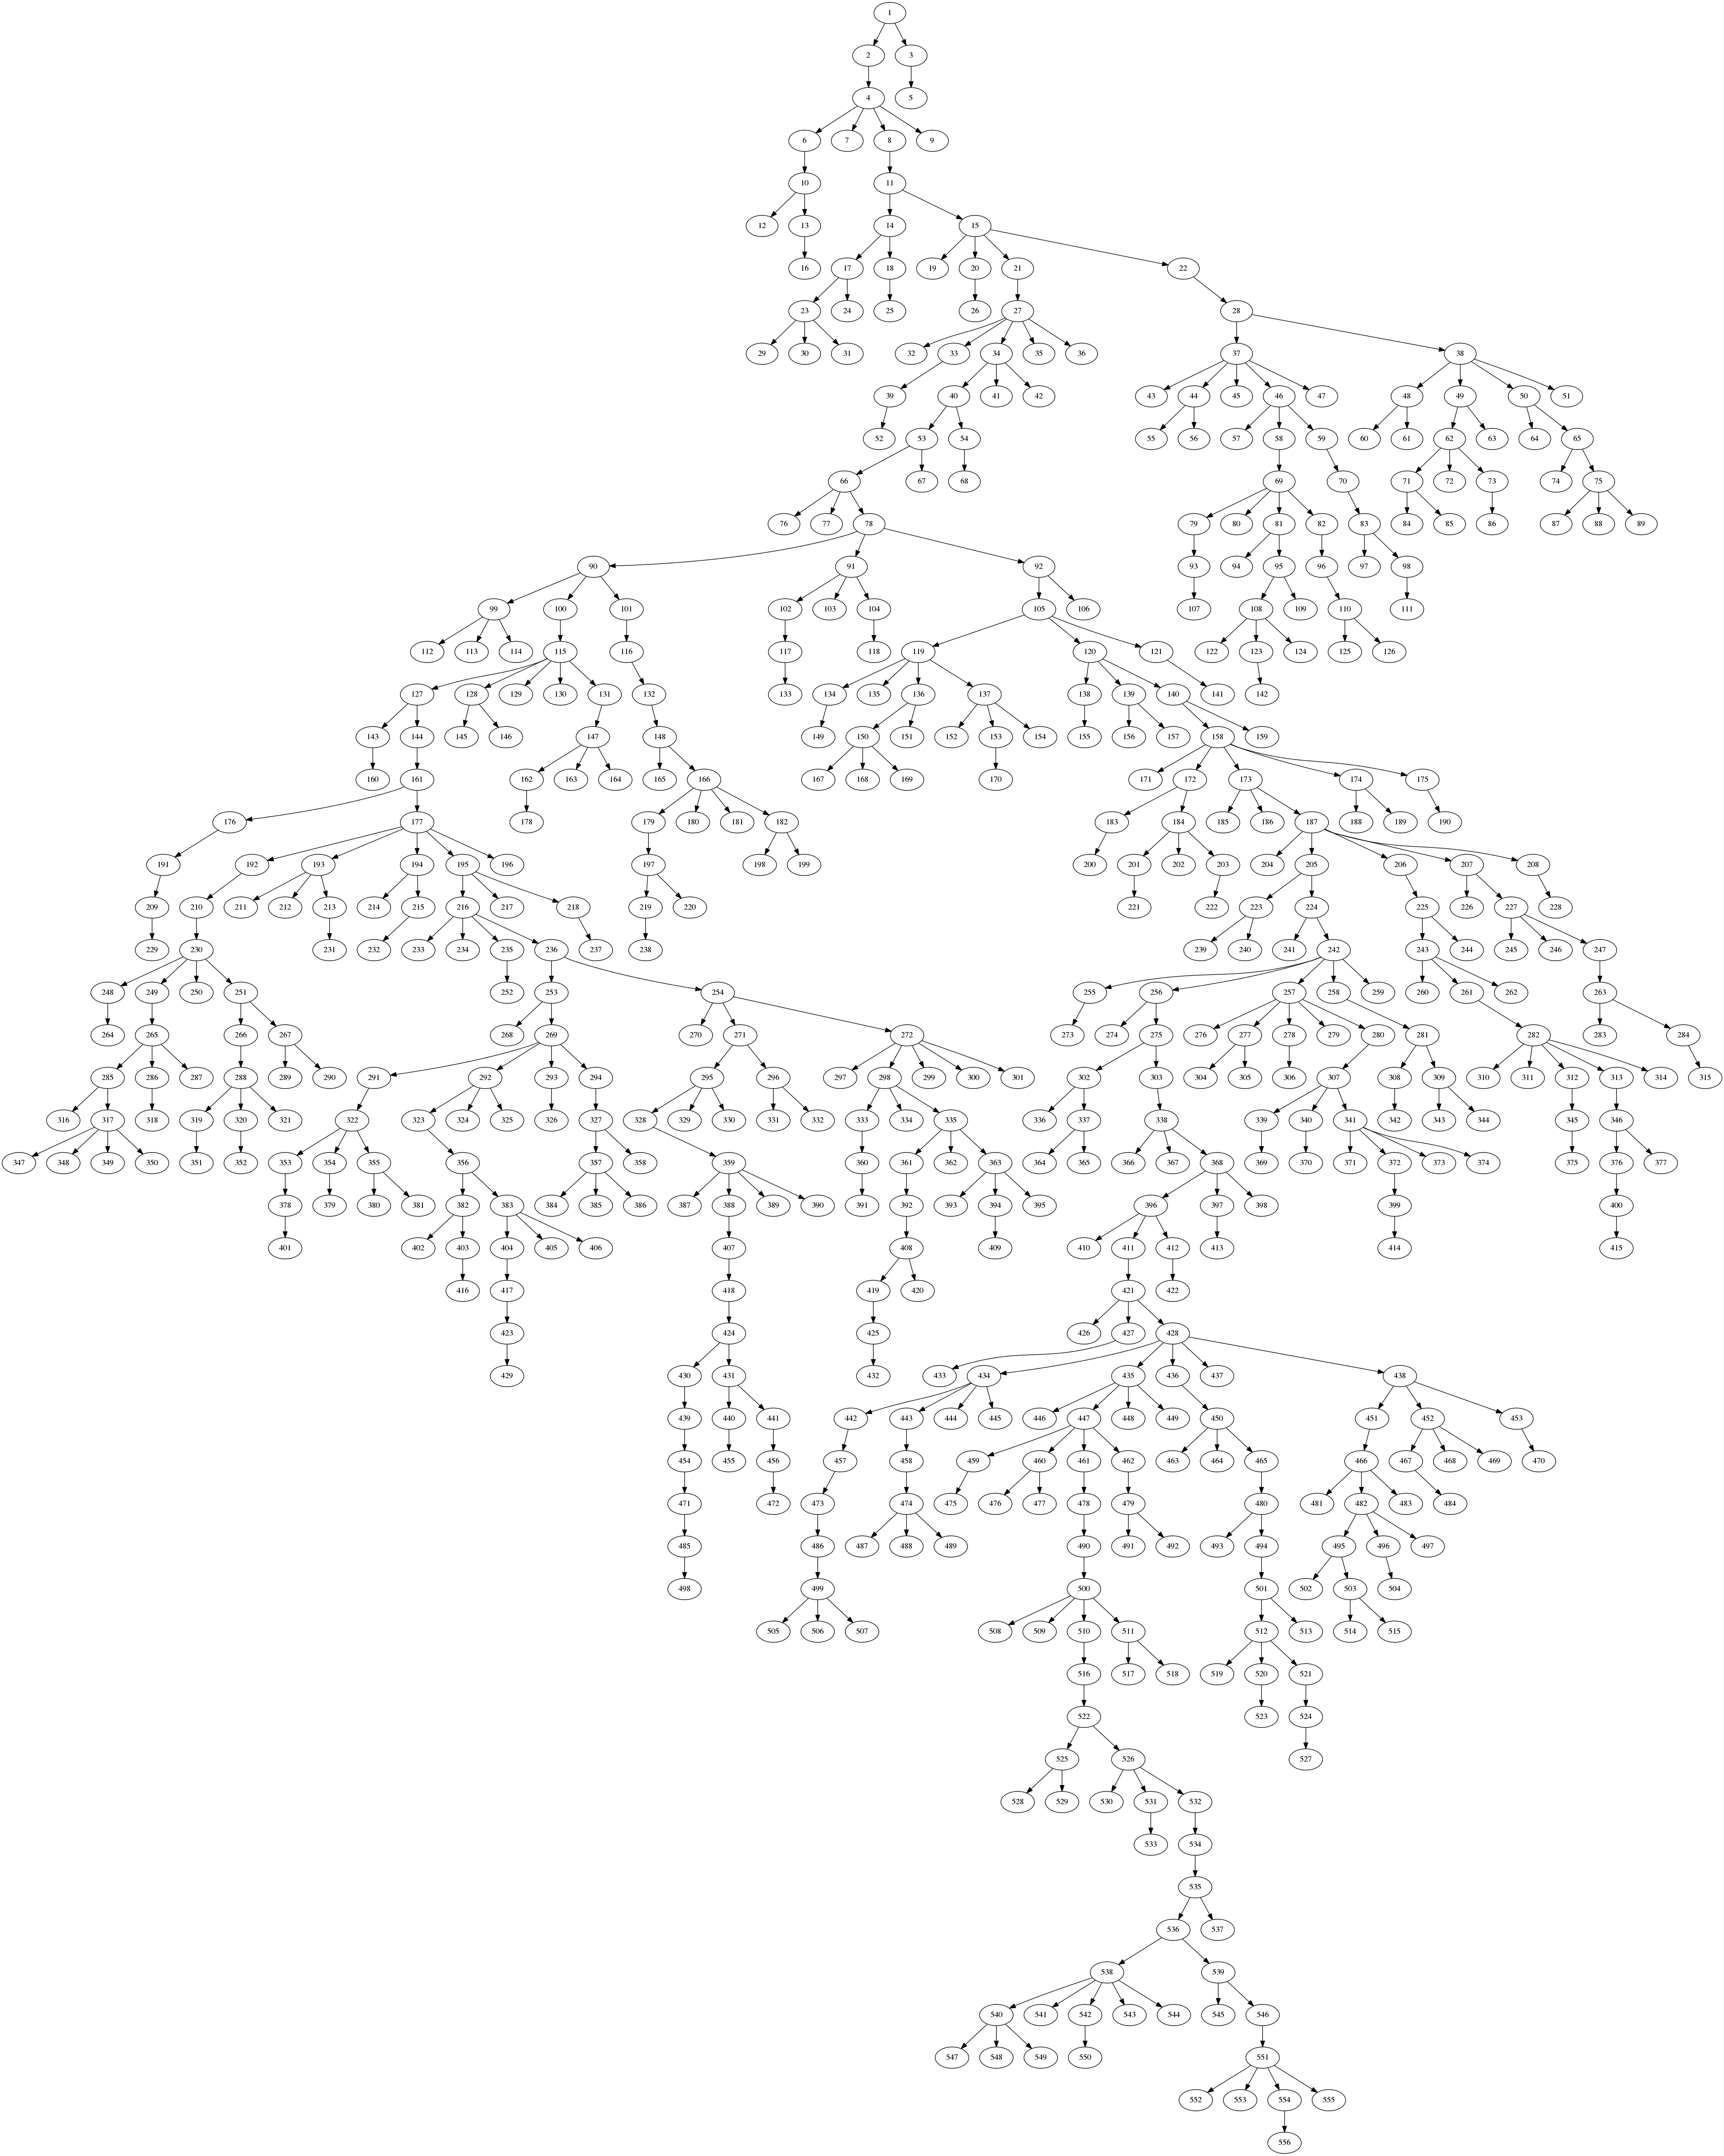
\includegraphics[width=10cm,height=6cm]{renduGV}
\end{center}
\end{figure}

\paragraph{TikZ}

\begin{figure}[h!] \centering \resizebox {6cm}{10cm} {
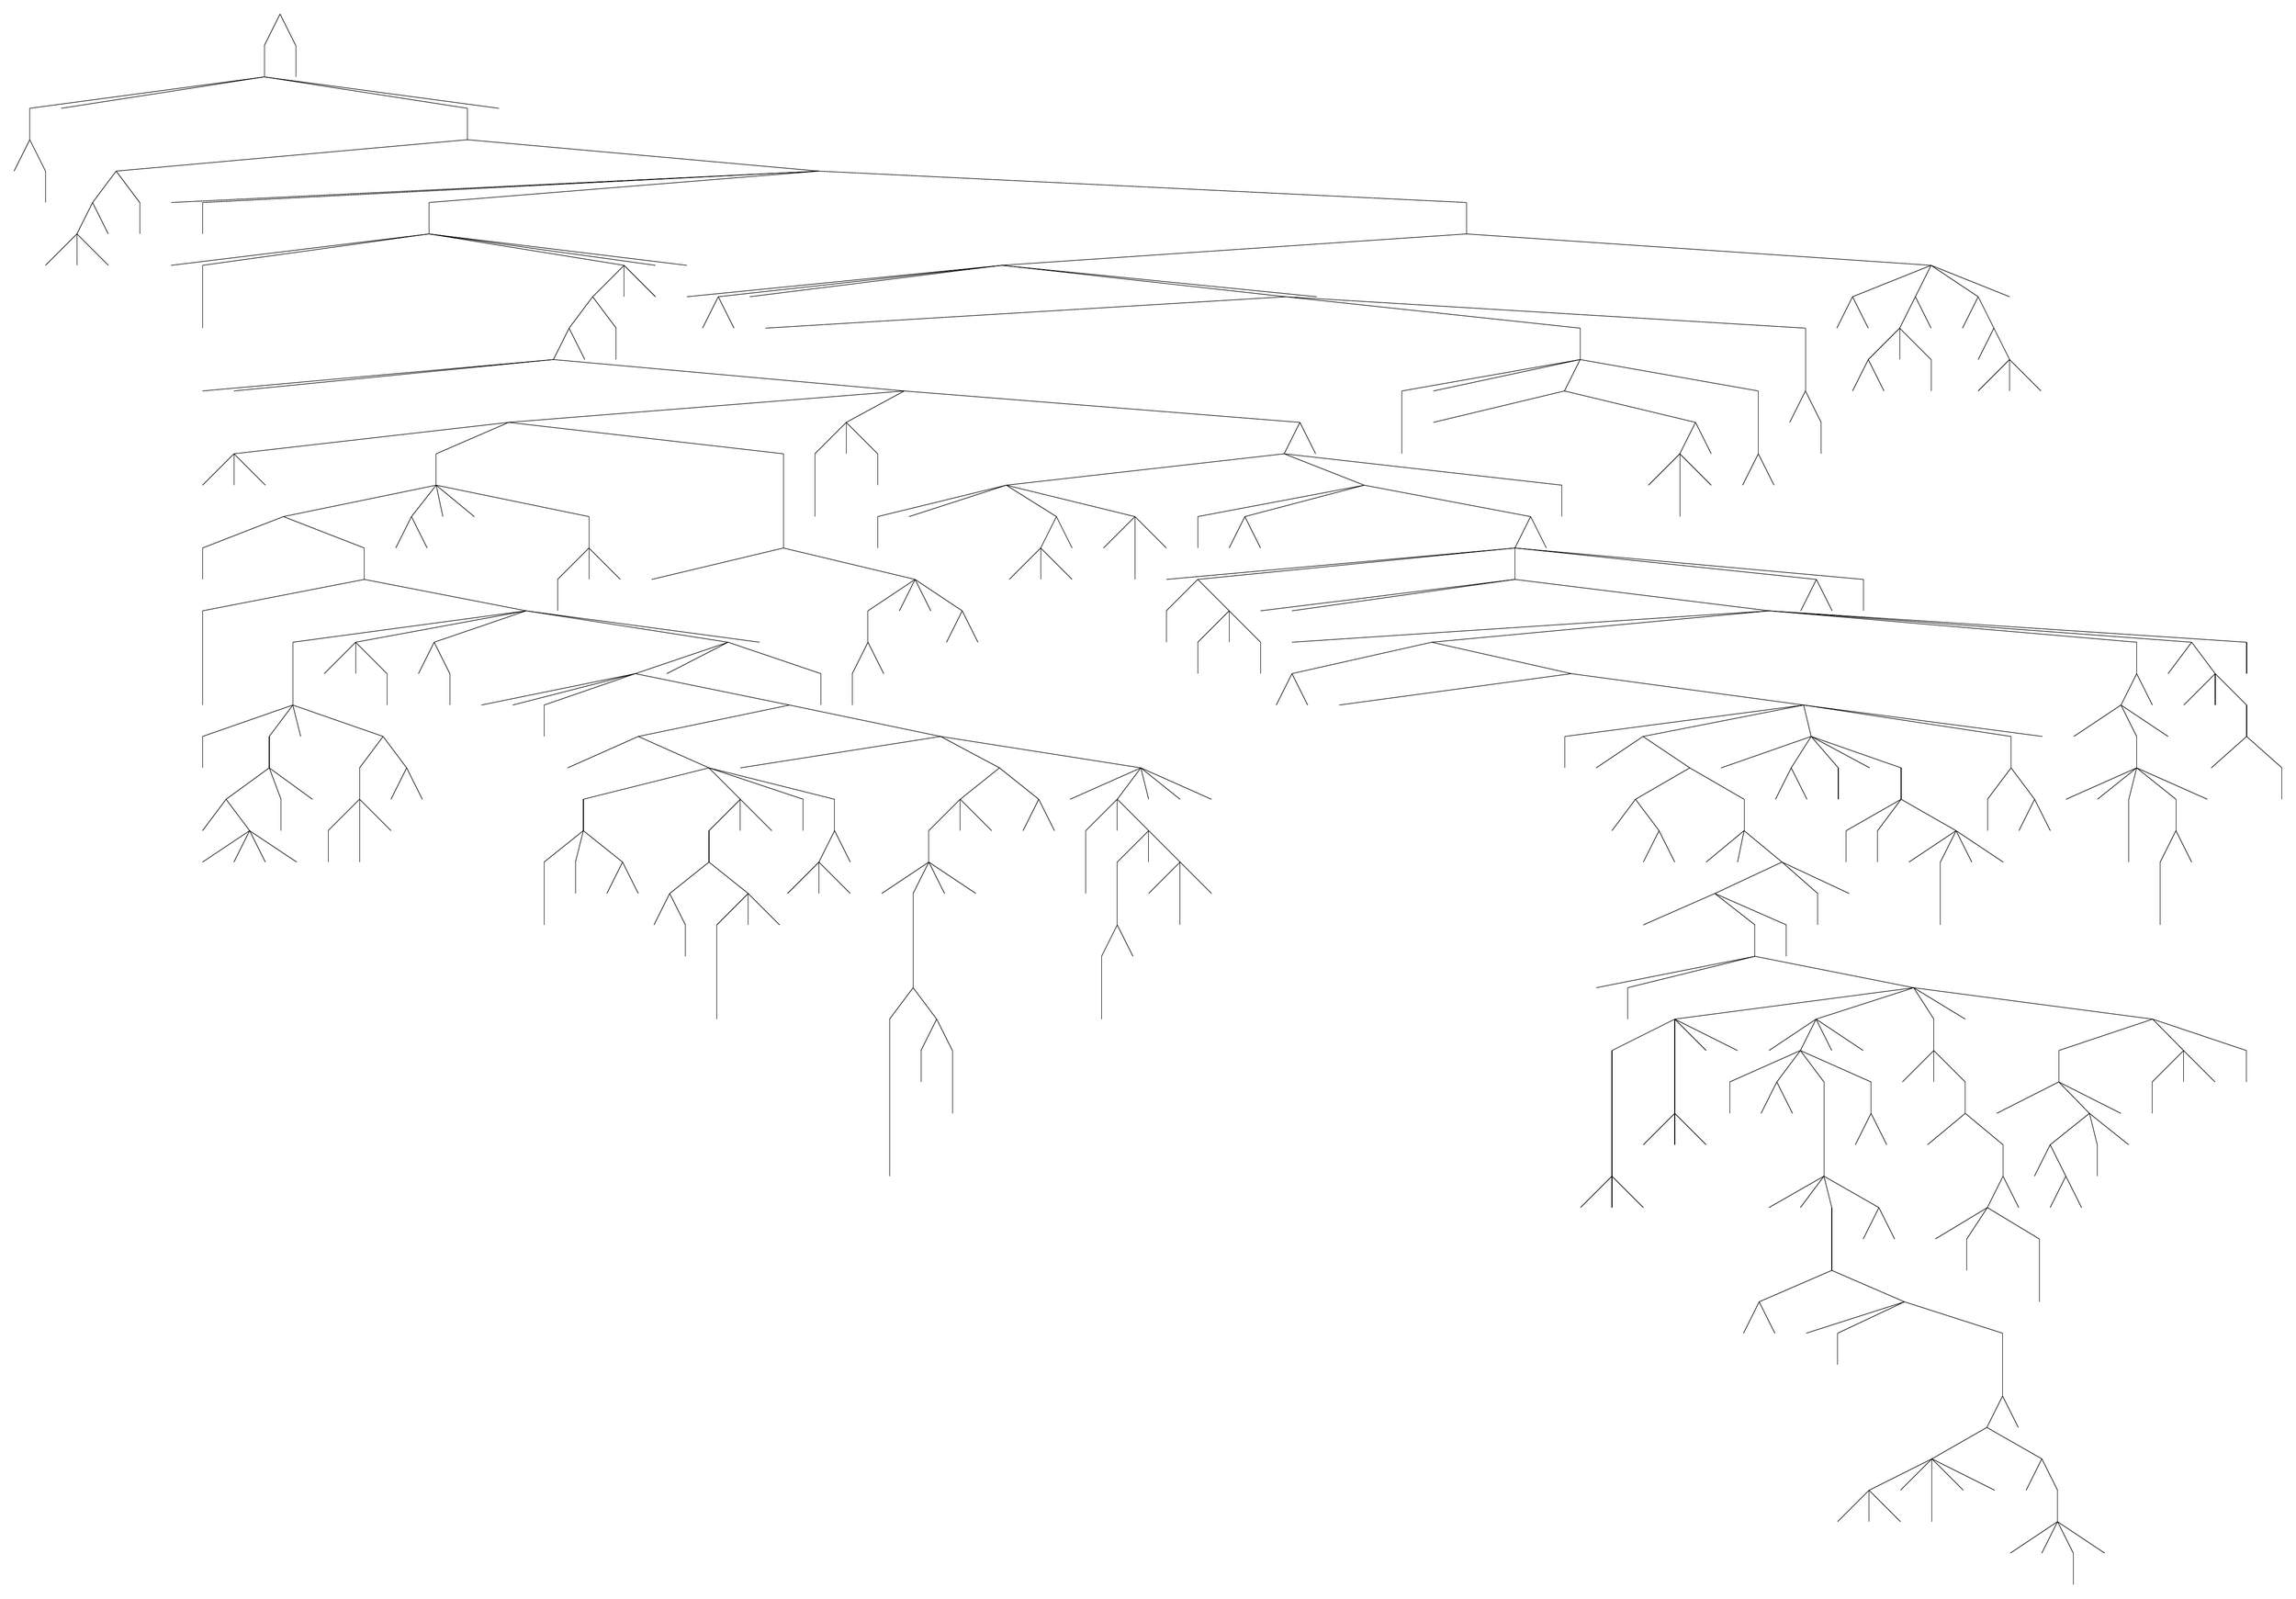
\begin{tikzpicture}[scale=0.8, every node/.style={scale=0.8}, node distance=1pt]
\draw (0.500000, -4.000000) -- (0.000000, -5.000000);
\draw (1.000000, -5.000000) -- (1.000000, -6.000000);
\draw (0.500000, -4.000000) -- (1.000000, -5.000000);
\draw (0.500000, -3.000000) -- (0.500000, -4.000000);
\draw (7.967918, -2.000000) -- (0.500000, -3.000000);
\draw (7.967918, -2.000000) -- (1.500000, -3.000000);
\draw (2.000000, -7.000000) -- (1.000000, -8.000000);
\draw (2.000000, -7.000000) -- (2.000000, -8.000000);
\draw (2.000000, -7.000000) -- (3.000000, -8.000000);
\draw (2.500000, -6.000000) -- (2.000000, -7.000000);
\draw (2.500000, -6.000000) -- (3.000000, -7.000000);
\draw (3.250000, -5.000000) -- (2.500000, -6.000000);
\draw (4.000000, -6.000000) -- (4.000000, -7.000000);
\draw (3.250000, -5.000000) -- (4.000000, -6.000000);
\draw (14.435836, -4.000000) -- (3.250000, -5.000000);
\draw (25.621671, -5.000000) -- (5.000000, -6.000000);
\draw (6.000000, -6.000000) -- (6.000000, -7.000000);
\draw (25.621671, -5.000000) -- (6.000000, -6.000000);
\draw (13.210886, -7.000000) -- (5.000000, -8.000000);
\draw (6.000000, -9.000000) -- (6.000000, -10.000000);
\draw (6.000000, -8.000000) -- (6.000000, -9.000000);
\draw (13.210886, -7.000000) -- (6.000000, -8.000000);
\draw (17.171772, -11.000000) -- (6.000000, -12.000000);
\draw (17.171772, -11.000000) -- (7.000000, -12.000000);
\draw (7.000000, -14.000000) -- (6.000000, -15.000000);
\draw (7.000000, -14.000000) -- (7.000000, -15.000000);
\draw (7.000000, -14.000000) -- (8.000000, -15.000000);
\draw (15.748047, -13.000000) -- (7.000000, -14.000000);
\draw (6.000000, -17.000000) -- (6.000000, -18.000000);
\draw (8.576172, -16.000000) -- (6.000000, -17.000000);
\draw (6.000000, -21.000000) -- (6.000000, -22.000000);
\draw (6.000000, -20.000000) -- (6.000000, -21.000000);
\draw (6.000000, -19.000000) -- (6.000000, -20.000000);
\draw (11.152344, -18.000000) -- (6.000000, -19.000000);
\draw (6.000000, -23.000000) -- (6.000000, -24.000000);
\draw (8.875000, -22.000000) -- (6.000000, -23.000000);
\draw (6.750000, -25.000000) -- (6.000000, -26.000000);
\draw (7.500000, -26.000000) -- (6.000000, -27.000000);
\draw (7.500000, -26.000000) -- (7.000000, -27.000000);
\draw (7.500000, -26.000000) -- (8.000000, -27.000000);
\draw (7.500000, -26.000000) -- (9.000000, -27.000000);
\draw (6.750000, -25.000000) -- (7.500000, -26.000000);
\draw (8.125000, -24.000000) -- (6.750000, -25.000000);
\draw (8.500000, -25.000000) -- (8.500000, -26.000000);
\draw (8.125000, -24.000000) -- (8.500000, -25.000000);
\draw (8.125000, -24.000000) -- (9.500000, -25.000000);
\draw (8.125000, -23.000000) -- (8.125000, -24.000000);
\draw (8.875000, -22.000000) -- (8.125000, -23.000000);
\draw (8.875000, -22.000000) -- (9.125000, -23.000000);
\draw (10.000000, -26.000000) -- (10.000000, -27.000000);
\draw (11.000000, -25.000000) -- (10.000000, -26.000000);
\draw (11.000000, -26.000000) -- (11.000000, -27.000000);
\draw (11.000000, -25.000000) -- (11.000000, -26.000000);
\draw (11.000000, -25.000000) -- (12.000000, -26.000000);
\draw (11.000000, -24.000000) -- (11.000000, -25.000000);
\draw (11.750000, -23.000000) -- (11.000000, -24.000000);
\draw (12.500000, -24.000000) -- (12.000000, -25.000000);
\draw (12.500000, -24.000000) -- (13.000000, -25.000000);
\draw (11.750000, -23.000000) -- (12.500000, -24.000000);
\draw (8.875000, -22.000000) -- (11.750000, -23.000000);
\draw (8.875000, -21.000000) -- (8.875000, -22.000000);
\draw (8.875000, -20.000000) -- (8.875000, -21.000000);
\draw (16.304688, -19.000000) -- (8.875000, -20.000000);
\draw (10.875000, -20.000000) -- (9.875000, -21.000000);
\draw (10.875000, -20.000000) -- (10.875000, -21.000000);
\draw (11.875000, -21.000000) -- (11.875000, -22.000000);
\draw (10.875000, -20.000000) -- (11.875000, -21.000000);
\draw (16.304688, -19.000000) -- (10.875000, -20.000000);
\draw (13.375000, -20.000000) -- (12.875000, -21.000000);
\draw (13.875000, -21.000000) -- (13.875000, -22.000000);
\draw (13.375000, -20.000000) -- (13.875000, -21.000000);
\draw (16.304688, -19.000000) -- (13.375000, -20.000000);
\draw (19.781250, -21.000000) -- (14.875000, -22.000000);
\draw (19.781250, -21.000000) -- (15.875000, -22.000000);
\draw (16.875000, -22.000000) -- (16.875000, -23.000000);
\draw (19.781250, -21.000000) -- (16.875000, -22.000000);
\draw (19.875000, -23.000000) -- (17.625000, -24.000000);
\draw (16.875000, -28.000000) -- (16.875000, -29.000000);
\draw (16.875000, -27.000000) -- (16.875000, -28.000000);
\draw (18.125000, -26.000000) -- (16.875000, -27.000000);
\draw (17.875000, -27.000000) -- (17.875000, -28.000000);
\draw (18.125000, -26.000000) -- (17.875000, -27.000000);
\draw (19.375000, -27.000000) -- (18.875000, -28.000000);
\draw (19.375000, -27.000000) -- (19.875000, -28.000000);
\draw (18.125000, -26.000000) -- (19.375000, -27.000000);
\draw (18.125000, -25.000000) -- (18.125000, -26.000000);
\draw (22.125000, -24.000000) -- (18.125000, -25.000000);
\draw (20.875000, -28.000000) -- (20.375000, -29.000000);
\draw (21.375000, -29.000000) -- (21.375000, -30.000000);
\draw (20.875000, -28.000000) -- (21.375000, -29.000000);
\draw (22.125000, -27.000000) -- (20.875000, -28.000000);
\draw (22.375000, -31.000000) -- (22.375000, -32.000000);
\draw (22.375000, -30.000000) -- (22.375000, -31.000000);
\draw (22.375000, -29.000000) -- (22.375000, -30.000000);
\draw (23.375000, -28.000000) -- (22.375000, -29.000000);
\draw (23.375000, -28.000000) -- (23.375000, -29.000000);
\draw (23.375000, -28.000000) -- (24.375000, -29.000000);
\draw (22.125000, -27.000000) -- (23.375000, -28.000000);
\draw (22.125000, -26.000000) -- (22.125000, -27.000000);
\draw (23.125000, -25.000000) -- (22.125000, -26.000000);
\draw (23.125000, -25.000000) -- (23.125000, -26.000000);
\draw (23.125000, -25.000000) -- (24.125000, -26.000000);
\draw (22.125000, -24.000000) -- (23.125000, -25.000000);
\draw (25.125000, -25.000000) -- (25.125000, -26.000000);
\draw (22.125000, -24.000000) -- (25.125000, -25.000000);
\draw (25.625000, -27.000000) -- (24.625000, -28.000000);
\draw (25.625000, -27.000000) -- (25.625000, -28.000000);
\draw (25.625000, -27.000000) -- (26.625000, -28.000000);
\draw (26.125000, -26.000000) -- (25.625000, -27.000000);
\draw (26.125000, -26.000000) -- (26.625000, -27.000000);
\draw (26.125000, -25.000000) -- (26.125000, -26.000000);
\draw (22.125000, -24.000000) -- (26.125000, -25.000000);
\draw (19.875000, -23.000000) -- (22.125000, -24.000000);
\draw (24.687500, -22.000000) -- (19.875000, -23.000000);
\draw (29.500000, -23.000000) -- (23.125000, -24.000000);
\draw (29.125000, -27.000000) -- (27.625000, -28.000000);
\draw (27.875000, -36.000000) -- (27.875000, -37.000000);
\draw (27.875000, -35.000000) -- (27.875000, -36.000000);
\draw (27.875000, -34.000000) -- (27.875000, -35.000000);
\draw (27.875000, -33.000000) -- (27.875000, -34.000000);
\draw (27.875000, -32.000000) -- (27.875000, -33.000000);
\draw (28.625000, -31.000000) -- (27.875000, -32.000000);
\draw (28.875000, -33.000000) -- (28.875000, -34.000000);
\draw (29.375000, -32.000000) -- (28.875000, -33.000000);
\draw (29.875000, -34.000000) -- (29.875000, -35.000000);
\draw (29.875000, -33.000000) -- (29.875000, -34.000000);
\draw (29.375000, -32.000000) -- (29.875000, -33.000000);
\draw (28.625000, -31.000000) -- (29.375000, -32.000000);
\draw (28.625000, -30.000000) -- (28.625000, -31.000000);
\draw (28.625000, -29.000000) -- (28.625000, -30.000000);
\draw (28.625000, -28.000000) -- (28.625000, -29.000000);
\draw (29.125000, -27.000000) -- (28.625000, -28.000000);
\draw (29.125000, -27.000000) -- (29.625000, -28.000000);
\draw (29.125000, -27.000000) -- (30.625000, -28.000000);
\draw (29.125000, -26.000000) -- (29.125000, -27.000000);
\draw (30.125000, -25.000000) -- (29.125000, -26.000000);
\draw (30.125000, -25.000000) -- (30.125000, -26.000000);
\draw (30.125000, -25.000000) -- (31.125000, -26.000000);
\draw (31.375000, -24.000000) -- (30.125000, -25.000000);
\draw (32.625000, -25.000000) -- (32.125000, -26.000000);
\draw (32.625000, -25.000000) -- (33.125000, -26.000000);
\draw (31.375000, -24.000000) -- (32.625000, -25.000000);
\draw (29.500000, -23.000000) -- (31.375000, -24.000000);
\draw (35.875000, -24.000000) -- (33.625000, -25.000000);
\draw (34.125000, -27.000000) -- (34.125000, -28.000000);
\draw (34.125000, -26.000000) -- (34.125000, -27.000000);
\draw (35.125000, -25.000000) -- (34.125000, -26.000000);
\draw (35.125000, -25.000000) -- (35.125000, -26.000000);
\draw (34.625000, -31.000000) -- (34.625000, -32.000000);
\draw (34.625000, -30.000000) -- (34.625000, -31.000000);
\draw (35.125000, -29.000000) -- (34.625000, -30.000000);
\draw (35.125000, -29.000000) -- (35.625000, -30.000000);
\draw (35.125000, -28.000000) -- (35.125000, -29.000000);
\draw (35.125000, -27.000000) -- (35.125000, -28.000000);
\draw (36.125000, -26.000000) -- (35.125000, -27.000000);
\draw (36.125000, -26.000000) -- (36.125000, -27.000000);
\draw (37.125000, -27.000000) -- (36.125000, -28.000000);
\draw (37.125000, -28.000000) -- (37.125000, -29.000000);
\draw (37.125000, -27.000000) -- (37.125000, -28.000000);
\draw (37.125000, -27.000000) -- (38.125000, -28.000000);
\draw (36.125000, -26.000000) -- (37.125000, -27.000000);
\draw (35.125000, -25.000000) -- (36.125000, -26.000000);
\draw (35.875000, -24.000000) -- (35.125000, -25.000000);
\draw (35.875000, -24.000000) -- (36.125000, -25.000000);
\draw (35.875000, -24.000000) -- (37.125000, -25.000000);
\draw (35.875000, -24.000000) -- (38.125000, -25.000000);
\draw (29.500000, -23.000000) -- (35.875000, -24.000000);
\draw (24.687500, -22.000000) -- (29.500000, -23.000000);
\draw (19.781250, -21.000000) -- (24.687500, -22.000000);
\draw (22.734375, -20.000000) -- (19.781250, -21.000000);
\draw (22.734375, -20.000000) -- (20.781250, -21.000000);
\draw (25.687500, -21.000000) -- (25.687500, -22.000000);
\draw (22.734375, -20.000000) -- (25.687500, -21.000000);
\draw (16.304688, -19.000000) -- (22.734375, -20.000000);
\draw (16.304688, -19.000000) -- (23.734375, -20.000000);
\draw (11.152344, -18.000000) -- (16.304688, -19.000000);
\draw (11.152344, -17.000000) -- (11.152344, -18.000000);
\draw (8.576172, -16.000000) -- (11.152344, -17.000000);
\draw (13.440430, -15.000000) -- (8.576172, -16.000000);
\draw (12.652344, -16.000000) -- (12.152344, -17.000000);
\draw (12.652344, -16.000000) -- (13.152344, -17.000000);
\draw (13.440430, -15.000000) -- (12.652344, -16.000000);
\draw (13.440430, -15.000000) -- (13.652344, -16.000000);
\draw (13.440430, -15.000000) -- (14.652344, -16.000000);
\draw (17.304688, -18.000000) -- (17.304688, -19.000000);
\draw (18.304688, -17.000000) -- (17.304688, -18.000000);
\draw (18.304688, -17.000000) -- (18.304688, -18.000000);
\draw (18.304688, -17.000000) -- (19.304688, -18.000000);
\draw (18.304688, -16.000000) -- (18.304688, -17.000000);
\draw (13.440430, -15.000000) -- (18.304688, -16.000000);
\draw (13.440430, -14.000000) -- (13.440430, -15.000000);
\draw (15.748047, -13.000000) -- (13.440430, -14.000000);
\draw (24.496094, -17.000000) -- (20.304688, -18.000000);
\draw (26.687500, -21.000000) -- (26.687500, -22.000000);
\draw (27.187500, -20.000000) -- (26.687500, -21.000000);
\draw (27.187500, -20.000000) -- (27.687500, -21.000000);
\draw (27.187500, -19.000000) -- (27.187500, -20.000000);
\draw (28.687500, -18.000000) -- (27.187500, -19.000000);
\draw (28.687500, -18.000000) -- (28.187500, -19.000000);
\draw (28.687500, -18.000000) -- (29.187500, -19.000000);
\draw (30.187500, -19.000000) -- (29.687500, -20.000000);
\draw (30.187500, -19.000000) -- (30.687500, -20.000000);
\draw (28.687500, -18.000000) -- (30.187500, -19.000000);
\draw (24.496094, -17.000000) -- (28.687500, -18.000000);
\draw (24.496094, -16.000000) -- (24.496094, -17.000000);
\draw (24.496094, -15.000000) -- (24.496094, -16.000000);
\draw (24.496094, -14.000000) -- (24.496094, -15.000000);
\draw (15.748047, -13.000000) -- (24.496094, -14.000000);
\draw (28.343544, -12.000000) -- (15.748047, -13.000000);
\draw (25.496094, -15.000000) -- (25.496094, -16.000000);
\draw (25.496094, -14.000000) -- (25.496094, -15.000000);
\draw (26.496094, -13.000000) -- (25.496094, -14.000000);
\draw (26.496094, -13.000000) -- (26.496094, -14.000000);
\draw (27.496094, -14.000000) -- (27.496094, -15.000000);
\draw (26.496094, -13.000000) -- (27.496094, -14.000000);
\draw (28.343544, -12.000000) -- (26.496094, -13.000000);
\draw (27.496094, -16.000000) -- (27.496094, -17.000000);
\draw (31.591797, -15.000000) -- (27.496094, -16.000000);
\draw (31.591797, -15.000000) -- (28.496094, -16.000000);
\draw (32.687500, -17.000000) -- (31.687500, -18.000000);
\draw (32.687500, -17.000000) -- (32.687500, -18.000000);
\draw (32.687500, -17.000000) -- (33.687500, -18.000000);
\draw (33.187500, -16.000000) -- (32.687500, -17.000000);
\draw (33.187500, -16.000000) -- (33.687500, -17.000000);
\draw (31.591797, -15.000000) -- (33.187500, -16.000000);
\draw (35.687500, -16.000000) -- (34.687500, -17.000000);
\draw (35.687500, -17.000000) -- (35.687500, -18.000000);
\draw (35.687500, -16.000000) -- (35.687500, -17.000000);
\draw (35.687500, -16.000000) -- (36.687500, -17.000000);
\draw (31.591797, -15.000000) -- (35.687500, -16.000000);
\draw (40.439041, -14.000000) -- (31.591797, -15.000000);
\draw (37.687500, -16.000000) -- (37.687500, -17.000000);
\draw (42.986893, -15.000000) -- (37.687500, -16.000000);
\draw (39.187500, -16.000000) -- (38.687500, -17.000000);
\draw (39.187500, -16.000000) -- (39.687500, -17.000000);
\draw (42.986893, -15.000000) -- (39.187500, -16.000000);
\draw (47.786285, -17.000000) -- (36.687500, -18.000000);
\draw (36.687500, -19.000000) -- (36.687500, -20.000000);
\draw (37.687500, -18.000000) -- (36.687500, -19.000000);
\draw (37.687500, -20.000000) -- (37.687500, -21.000000);
\draw (38.687500, -19.000000) -- (37.687500, -20.000000);
\draw (38.687500, -19.000000) -- (38.687500, -20.000000);
\draw (39.687500, -20.000000) -- (39.687500, -21.000000);
\draw (38.687500, -19.000000) -- (39.687500, -20.000000);
\draw (37.687500, -18.000000) -- (38.687500, -19.000000);
\draw (47.786285, -17.000000) -- (37.687500, -18.000000);
\draw (47.786285, -18.000000) -- (39.687500, -19.000000);
\draw (47.786285, -18.000000) -- (40.687500, -19.000000);
\draw (55.885071, -19.000000) -- (40.687500, -20.000000);
\draw (40.687500, -21.000000) -- (40.187500, -22.000000);
\draw (40.687500, -21.000000) -- (41.187500, -22.000000);
\draw (45.135330, -20.000000) -- (40.687500, -21.000000);
\draw (49.583160, -21.000000) -- (42.187500, -22.000000);
\draw (49.375000, -23.000000) -- (49.375000, -24.000000);
\draw (56.978821, -22.000000) -- (49.375000, -23.000000);
\draw (51.864410, -23.000000) -- (50.375000, -24.000000);
\draw (51.625000, -25.000000) -- (50.875000, -26.000000);
\draw (52.375000, -26.000000) -- (51.875000, -27.000000);
\draw (52.375000, -26.000000) -- (52.875000, -27.000000);
\draw (51.625000, -25.000000) -- (52.375000, -26.000000);
\draw (53.353821, -24.000000) -- (51.625000, -25.000000);
\draw (55.082642, -26.000000) -- (53.875000, -27.000000);
\draw (55.082642, -26.000000) -- (54.875000, -27.000000);
\draw (54.151855, -28.000000) -- (51.875000, -29.000000);
\draw (55.428711, -30.000000) -- (50.375000, -31.000000);
\draw (51.375000, -31.000000) -- (51.375000, -32.000000);
\draw (55.428711, -30.000000) -- (51.375000, -31.000000);
\draw (50.875000, -37.000000) -- (49.875000, -38.000000);
\draw (50.875000, -37.000000) -- (50.875000, -38.000000);
\draw (50.875000, -37.000000) -- (51.875000, -38.000000);
\draw (50.875000, -36.000000) -- (50.875000, -37.000000);
\draw (50.875000, -35.000000) -- (50.875000, -36.000000);
\draw (50.875000, -34.000000) -- (50.875000, -35.000000);
\draw (50.875000, -33.000000) -- (50.875000, -34.000000);
\draw (52.875000, -32.000000) -- (50.875000, -33.000000);
\draw (52.875000, -35.000000) -- (51.875000, -36.000000);
\draw (52.875000, -35.000000) -- (52.875000, -36.000000);
\draw (52.875000, -35.000000) -- (53.875000, -36.000000);
\draw (52.875000, -34.000000) -- (52.875000, -35.000000);
\draw (52.875000, -33.000000) -- (52.875000, -34.000000);
\draw (52.875000, -32.000000) -- (52.875000, -33.000000);
\draw (52.875000, -32.000000) -- (53.875000, -33.000000);
\draw (52.875000, -32.000000) -- (54.875000, -33.000000);
\draw (60.482422, -31.000000) -- (52.875000, -32.000000);
\draw (57.375000, -32.000000) -- (55.875000, -33.000000);
\draw (54.625000, -34.000000) -- (54.625000, -35.000000);
\draw (56.875000, -33.000000) -- (54.625000, -34.000000);
\draw (56.125000, -34.000000) -- (55.625000, -35.000000);
\draw (56.125000, -34.000000) -- (56.625000, -35.000000);
\draw (56.875000, -33.000000) -- (56.125000, -34.000000);
\draw (57.625000, -37.000000) -- (55.875000, -38.000000);
\draw (57.625000, -37.000000) -- (56.875000, -38.000000);
\draw (55.562500, -41.000000) -- (55.062500, -42.000000);
\draw (55.562500, -41.000000) -- (56.062500, -42.000000);
\draw (57.875000, -40.000000) -- (55.562500, -41.000000);
\draw (60.187500, -41.000000) -- (57.062500, -42.000000);
\draw (58.062500, -42.000000) -- (58.062500, -43.000000);
\draw (60.187500, -41.000000) -- (58.062500, -42.000000);
\draw (59.062500, -47.000000) -- (58.062500, -48.000000);
\draw (59.062500, -47.000000) -- (59.062500, -48.000000);
\draw (59.062500, -47.000000) -- (60.062500, -48.000000);
\draw (61.062500, -46.000000) -- (59.062500, -47.000000);
\draw (61.062500, -46.000000) -- (60.062500, -47.000000);
\draw (61.062500, -47.000000) -- (61.062500, -48.000000);
\draw (61.062500, -46.000000) -- (61.062500, -47.000000);
\draw (61.062500, -46.000000) -- (62.062500, -47.000000);
\draw (61.062500, -46.000000) -- (63.062500, -47.000000);
\draw (62.812500, -45.000000) -- (61.062500, -46.000000);
\draw (64.562500, -46.000000) -- (64.062500, -47.000000);
\draw (65.062500, -48.000000) -- (63.562500, -49.000000);
\draw (65.062500, -48.000000) -- (64.562500, -49.000000);
\draw (65.562500, -49.000000) -- (65.562500, -50.000000);
\draw (65.062500, -48.000000) -- (65.562500, -49.000000);
\draw (65.062500, -48.000000) -- (66.562500, -49.000000);
\draw (65.062500, -47.000000) -- (65.062500, -48.000000);
\draw (64.562500, -46.000000) -- (65.062500, -47.000000);
\draw (62.812500, -45.000000) -- (64.562500, -46.000000);
\draw (63.312500, -44.000000) -- (62.812500, -45.000000);
\draw (63.312500, -44.000000) -- (63.812500, -45.000000);
\draw (63.312500, -43.000000) -- (63.312500, -44.000000);
\draw (63.312500, -42.000000) -- (63.312500, -43.000000);
\draw (60.187500, -41.000000) -- (63.312500, -42.000000);
\draw (57.875000, -40.000000) -- (60.187500, -41.000000);
\draw (57.875000, -39.000000) -- (57.875000, -40.000000);
\draw (57.875000, -38.000000) -- (57.875000, -39.000000);
\draw (57.625000, -37.000000) -- (57.875000, -38.000000);
\draw (59.375000, -38.000000) -- (58.875000, -39.000000);
\draw (59.375000, -38.000000) -- (59.875000, -39.000000);
\draw (57.625000, -37.000000) -- (59.375000, -38.000000);
\draw (57.625000, -36.000000) -- (57.625000, -37.000000);
\draw (57.625000, -35.000000) -- (57.625000, -36.000000);
\draw (57.625000, -34.000000) -- (57.625000, -35.000000);
\draw (56.875000, -33.000000) -- (57.625000, -34.000000);
\draw (59.125000, -35.000000) -- (58.625000, -36.000000);
\draw (59.125000, -35.000000) -- (59.625000, -36.000000);
\draw (59.125000, -34.000000) -- (59.125000, -35.000000);
\draw (56.875000, -33.000000) -- (59.125000, -34.000000);
\draw (57.375000, -32.000000) -- (56.875000, -33.000000);
\draw (57.375000, -32.000000) -- (57.875000, -33.000000);
\draw (57.375000, -32.000000) -- (58.875000, -33.000000);
\draw (60.482422, -31.000000) -- (57.375000, -32.000000);
\draw (61.125000, -33.000000) -- (60.125000, -34.000000);
\draw (61.125000, -33.000000) -- (61.125000, -34.000000);
\draw (62.125000, -35.000000) -- (60.921875, -36.000000);
\draw (62.828125, -38.000000) -- (61.171875, -39.000000);
\draw (62.171875, -39.000000) -- (62.171875, -40.000000);
\draw (62.828125, -38.000000) -- (62.171875, -39.000000);
\draw (64.484375, -40.000000) -- (64.484375, -41.000000);
\draw (64.484375, -39.000000) -- (64.484375, -40.000000);
\draw (62.828125, -38.000000) -- (64.484375, -39.000000);
\draw (63.328125, -37.000000) -- (62.828125, -38.000000);
\draw (63.328125, -37.000000) -- (63.828125, -38.000000);
\draw (63.328125, -36.000000) -- (63.328125, -37.000000);
\draw (62.125000, -35.000000) -- (63.328125, -36.000000);
\draw (62.125000, -34.000000) -- (62.125000, -35.000000);
\draw (61.125000, -33.000000) -- (62.125000, -34.000000);
\draw (61.125000, -32.000000) -- (61.125000, -33.000000);
\draw (60.482422, -31.000000) -- (61.125000, -32.000000);
\draw (60.482422, -31.000000) -- (62.125000, -32.000000);
\draw (65.101562, -34.000000) -- (63.125000, -35.000000);
\draw (64.828125, -36.000000) -- (64.328125, -37.000000);
\draw (65.328125, -37.000000) -- (64.828125, -38.000000);
\draw (65.328125, -37.000000) -- (65.828125, -38.000000);
\draw (64.828125, -36.000000) -- (65.328125, -37.000000);
\draw (66.078125, -35.000000) -- (64.828125, -36.000000);
\draw (66.328125, -36.000000) -- (66.328125, -37.000000);
\draw (66.078125, -35.000000) -- (66.328125, -36.000000);
\draw (66.078125, -35.000000) -- (67.328125, -36.000000);
\draw (65.101562, -34.000000) -- (66.078125, -35.000000);
\draw (65.101562, -34.000000) -- (67.078125, -35.000000);
\draw (65.101562, -33.000000) -- (65.101562, -34.000000);
\draw (68.089844, -32.000000) -- (65.101562, -33.000000);
\draw (68.078125, -34.000000) -- (68.078125, -35.000000);
\draw (69.078125, -33.000000) -- (68.078125, -34.000000);
\draw (69.078125, -33.000000) -- (69.078125, -34.000000);
\draw (69.078125, -33.000000) -- (70.078125, -34.000000);
\draw (68.089844, -32.000000) -- (69.078125, -33.000000);
\draw (71.078125, -33.000000) -- (71.078125, -34.000000);
\draw (68.089844, -32.000000) -- (71.078125, -33.000000);
\draw (60.482422, -31.000000) -- (68.089844, -32.000000);
\draw (55.428711, -30.000000) -- (60.482422, -31.000000);
\draw (55.428711, -29.000000) -- (55.428711, -30.000000);
\draw (54.151855, -28.000000) -- (55.428711, -29.000000);
\draw (56.428711, -29.000000) -- (56.428711, -30.000000);
\draw (54.151855, -28.000000) -- (56.428711, -29.000000);
\draw (56.290283, -27.000000) -- (54.151855, -28.000000);
\draw (57.428711, -28.000000) -- (57.428711, -29.000000);
\draw (56.290283, -27.000000) -- (57.428711, -28.000000);
\draw (56.290283, -27.000000) -- (58.428711, -28.000000);
\draw (55.082642, -26.000000) -- (56.290283, -27.000000);
\draw (55.082642, -25.000000) -- (55.082642, -26.000000);
\draw (53.353821, -24.000000) -- (55.082642, -25.000000);
\draw (51.864410, -23.000000) -- (53.353821, -24.000000);
\draw (56.978821, -22.000000) -- (51.864410, -23.000000);
\draw (57.218231, -23.000000) -- (54.353821, -24.000000);
\draw (56.582642, -24.000000) -- (56.082642, -25.000000);
\draw (56.582642, -24.000000) -- (57.082642, -25.000000);
\draw (57.218231, -23.000000) -- (56.582642, -24.000000);
\draw (58.082642, -24.000000) -- (58.082642, -25.000000);
\draw (57.218231, -23.000000) -- (58.082642, -24.000000);
\draw (57.218231, -23.000000) -- (59.082642, -24.000000);
\draw (58.332642, -26.000000) -- (58.332642, -27.000000);
\draw (60.082642, -25.000000) -- (58.332642, -26.000000);
\draw (59.332642, -26.000000) -- (59.332642, -27.000000);
\draw (60.082642, -25.000000) -- (59.332642, -26.000000);
\draw (61.832642, -26.000000) -- (60.332642, -27.000000);
\draw (61.332642, -28.000000) -- (61.332642, -29.000000);
\draw (61.332642, -27.000000) -- (61.332642, -28.000000);
\draw (61.832642, -26.000000) -- (61.332642, -27.000000);
\draw (61.832642, -26.000000) -- (62.332642, -27.000000);
\draw (61.832642, -26.000000) -- (63.332642, -27.000000);
\draw (60.082642, -25.000000) -- (61.832642, -26.000000);
\draw (60.082642, -24.000000) -- (60.082642, -25.000000);
\draw (57.218231, -23.000000) -- (60.082642, -24.000000);
\draw (56.978821, -22.000000) -- (57.218231, -23.000000);
\draw (62.832642, -25.000000) -- (62.832642, -26.000000);
\draw (63.582642, -24.000000) -- (62.832642, -25.000000);
\draw (64.332642, -25.000000) -- (63.832642, -26.000000);
\draw (64.332642, -25.000000) -- (64.832642, -26.000000);
\draw (63.582642, -24.000000) -- (64.332642, -25.000000);
\draw (63.582642, -23.000000) -- (63.582642, -24.000000);
\draw (56.978821, -22.000000) -- (63.582642, -23.000000);
\draw (56.978821, -22.000000) -- (64.582642, -23.000000);
\draw (49.583160, -21.000000) -- (56.978821, -22.000000);
\draw (45.135330, -20.000000) -- (49.583160, -21.000000);
\draw (55.885071, -19.000000) -- (45.135330, -20.000000);
\draw (67.082642, -22.000000) -- (65.582642, -23.000000);
\draw (67.582642, -24.000000) -- (65.332642, -25.000000);
\draw (67.582642, -24.000000) -- (66.332642, -25.000000);
\draw (67.332642, -26.000000) -- (67.332642, -27.000000);
\draw (67.332642, -25.000000) -- (67.332642, -26.000000);
\draw (67.582642, -24.000000) -- (67.332642, -25.000000);
\draw (68.332642, -28.000000) -- (68.332642, -29.000000);
\draw (68.332642, -27.000000) -- (68.332642, -28.000000);
\draw (68.832642, -26.000000) -- (68.332642, -27.000000);
\draw (68.832642, -26.000000) -- (69.332642, -27.000000);
\draw (68.832642, -25.000000) -- (68.832642, -26.000000);
\draw (67.582642, -24.000000) -- (68.832642, -25.000000);
\draw (67.582642, -24.000000) -- (69.832642, -25.000000);
\draw (67.582642, -23.000000) -- (67.582642, -24.000000);
\draw (67.082642, -22.000000) -- (67.582642, -23.000000);
\draw (67.082642, -22.000000) -- (68.582642, -23.000000);
\draw (67.582642, -21.000000) -- (67.082642, -22.000000);
\draw (67.582642, -21.000000) -- (68.082642, -22.000000);
\draw (67.582642, -20.000000) -- (67.582642, -21.000000);
\draw (55.885071, -19.000000) -- (67.582642, -20.000000);
\draw (69.332642, -20.000000) -- (68.582642, -21.000000);
\draw (70.082642, -21.000000) -- (69.082642, -22.000000);
\draw (70.082642, -21.000000) -- (70.082642, -22.000000);
\draw (71.082642, -23.000000) -- (69.957642, -24.000000);
\draw (72.207642, -24.000000) -- (72.207642, -25.000000);
\draw (71.082642, -23.000000) -- (72.207642, -24.000000);
\draw (71.082642, -22.000000) -- (71.082642, -23.000000);
\draw (70.082642, -21.000000) -- (71.082642, -22.000000);
\draw (69.332642, -20.000000) -- (70.082642, -21.000000);
\draw (55.885071, -19.000000) -- (69.332642, -20.000000);
\draw (71.082642, -20.000000) -- (71.082642, -21.000000);
\draw (55.885071, -19.000000) -- (71.082642, -20.000000);
\draw (47.786285, -18.000000) -- (55.885071, -19.000000);
\draw (47.786285, -17.000000) -- (47.786285, -18.000000);
\draw (57.385071, -18.000000) -- (56.885071, -19.000000);
\draw (57.385071, -18.000000) -- (57.885071, -19.000000);
\draw (47.786285, -17.000000) -- (57.385071, -18.000000);
\draw (58.885071, -18.000000) -- (58.885071, -19.000000);
\draw (47.786285, -17.000000) -- (58.885071, -18.000000);
\draw (48.286285, -16.000000) -- (47.786285, -17.000000);
\draw (48.286285, -16.000000) -- (48.786285, -17.000000);
\draw (42.986893, -15.000000) -- (48.286285, -16.000000);
\draw (40.439041, -14.000000) -- (42.986893, -15.000000);
\draw (49.286285, -15.000000) -- (49.286285, -16.000000);
\draw (40.439041, -14.000000) -- (49.286285, -15.000000);
\draw (40.939041, -13.000000) -- (40.439041, -14.000000);
\draw (40.939041, -13.000000) -- (41.439041, -14.000000);
\draw (28.343544, -12.000000) -- (40.939041, -13.000000);
\draw (17.171772, -11.000000) -- (28.343544, -12.000000);
\draw (17.671772, -10.000000) -- (17.171772, -11.000000);
\draw (17.671772, -10.000000) -- (18.171772, -11.000000);
\draw (18.421772, -9.000000) -- (17.671772, -10.000000);
\draw (19.171772, -10.000000) -- (19.171772, -11.000000);
\draw (18.421772, -9.000000) -- (19.171772, -10.000000);
\draw (19.421772, -8.000000) -- (18.421772, -9.000000);
\draw (19.421772, -8.000000) -- (19.421772, -9.000000);
\draw (19.421772, -8.000000) -- (20.421772, -9.000000);
\draw (13.210886, -7.000000) -- (19.421772, -8.000000);
\draw (13.210886, -7.000000) -- (20.421772, -8.000000);
\draw (13.210886, -7.000000) -- (21.421772, -8.000000);
\draw (13.210886, -6.000000) -- (13.210886, -7.000000);
\draw (25.621671, -5.000000) -- (13.210886, -6.000000);
\draw (31.450400, -8.000000) -- (21.421772, -9.000000);
\draw (22.421772, -9.000000) -- (21.921772, -10.000000);
\draw (22.421772, -9.000000) -- (22.921772, -10.000000);
\draw (31.450400, -8.000000) -- (22.421772, -9.000000);
\draw (31.450400, -8.000000) -- (23.421772, -9.000000);
\draw (40.479029, -9.000000) -- (23.921772, -10.000000);
\draw (44.189041, -13.000000) -- (44.189041, -14.000000);
\draw (44.189041, -12.000000) -- (44.189041, -13.000000);
\draw (49.862663, -11.000000) -- (44.189041, -12.000000);
\draw (49.862663, -11.000000) -- (45.189041, -12.000000);
\draw (49.362663, -12.000000) -- (45.189041, -13.000000);
\draw (53.036285, -14.000000) -- (52.036285, -15.000000);
\draw (53.036285, -15.000000) -- (53.036285, -16.000000);
\draw (53.036285, -14.000000) -- (53.036285, -15.000000);
\draw (53.036285, -14.000000) -- (54.036285, -15.000000);
\draw (53.536285, -13.000000) -- (53.036285, -14.000000);
\draw (53.536285, -13.000000) -- (54.036285, -14.000000);
\draw (49.362663, -12.000000) -- (53.536285, -13.000000);
\draw (49.862663, -11.000000) -- (49.362663, -12.000000);
\draw (55.536285, -14.000000) -- (55.036285, -15.000000);
\draw (55.536285, -14.000000) -- (56.036285, -15.000000);
\draw (55.536285, -13.000000) -- (55.536285, -14.000000);
\draw (55.536285, -12.000000) -- (55.536285, -13.000000);
\draw (49.862663, -11.000000) -- (55.536285, -12.000000);
\draw (49.862663, -10.000000) -- (49.862663, -11.000000);
\draw (40.479029, -9.000000) -- (49.862663, -10.000000);
\draw (57.036285, -12.000000) -- (56.536285, -13.000000);
\draw (57.536285, -13.000000) -- (57.536285, -14.000000);
\draw (57.036285, -12.000000) -- (57.536285, -13.000000);
\draw (57.036285, -11.000000) -- (57.036285, -12.000000);
\draw (57.036285, -10.000000) -- (57.036285, -11.000000);
\draw (40.479029, -9.000000) -- (57.036285, -10.000000);
\draw (31.450400, -8.000000) -- (40.479029, -9.000000);
\draw (31.450400, -8.000000) -- (41.479029, -9.000000);
\draw (46.243343, -7.000000) -- (31.450400, -8.000000);
\draw (58.536285, -9.000000) -- (58.036285, -10.000000);
\draw (58.536285, -9.000000) -- (59.036285, -10.000000);
\draw (61.036285, -8.000000) -- (58.536285, -9.000000);
\draw (59.036285, -11.000000) -- (58.536285, -12.000000);
\draw (59.036285, -11.000000) -- (59.536285, -12.000000);
\draw (60.036285, -10.000000) -- (59.036285, -11.000000);
\draw (60.036285, -10.000000) -- (60.036285, -11.000000);
\draw (61.036285, -11.000000) -- (61.036285, -12.000000);
\draw (60.036285, -10.000000) -- (61.036285, -11.000000);
\draw (60.536285, -9.000000) -- (60.036285, -10.000000);
\draw (60.536285, -9.000000) -- (61.036285, -10.000000);
\draw (61.036285, -8.000000) -- (60.536285, -9.000000);
\draw (62.536285, -9.000000) -- (62.036285, -10.000000);
\draw (63.036285, -10.000000) -- (62.536285, -11.000000);
\draw (63.536285, -11.000000) -- (62.536285, -12.000000);
\draw (63.536285, -11.000000) -- (63.536285, -12.000000);
\draw (63.536285, -11.000000) -- (64.536285, -12.000000);
\draw (63.036285, -10.000000) -- (63.536285, -11.000000);
\draw (62.536285, -9.000000) -- (63.036285, -10.000000);
\draw (61.036285, -8.000000) -- (62.536285, -9.000000);
\draw (61.036285, -8.000000) -- (63.536285, -9.000000);
\draw (46.243343, -7.000000) -- (61.036285, -8.000000);
\draw (46.243343, -6.000000) -- (46.243343, -7.000000);
\draw (25.621671, -5.000000) -- (46.243343, -6.000000);
\draw (14.435836, -4.000000) -- (25.621671, -5.000000);
\draw (14.435836, -3.000000) -- (14.435836, -4.000000);
\draw (7.967918, -2.000000) -- (14.435836, -3.000000);
\draw (7.967918, -2.000000) -- (15.435836, -3.000000);
\draw (7.967918, -1.000000) -- (7.967918, -2.000000);
\draw (8.467918, -0.000000) -- (7.967918, -1.000000);
\draw (8.967918, -1.000000) -- (8.967918, -2.000000);
\draw (8.467918, -0.000000) -- (8.967918, -1.000000);

\end{tikzpicture}}
\end{figure}

\paragraph{Asymptote}

\begin{figure}[h!]
\begin{asy}
size(20cm, 20cm);
draw((0.500000, -4.000000) -- (0.000000, -5.000000));
draw((1.000000, -5.000000) -- (1.000000, -6.000000));
draw((0.500000, -4.000000) -- (1.000000, -5.000000));
draw((0.500000, -3.000000) -- (0.500000, -4.000000));
draw((7.967918, -2.000000) -- (0.500000, -3.000000));
draw((7.967918, -2.000000) -- (1.500000, -3.000000));
draw((2.000000, -7.000000) -- (1.000000, -8.000000));
draw((2.000000, -7.000000) -- (2.000000, -8.000000));
draw((2.000000, -7.000000) -- (3.000000, -8.000000));
draw((2.500000, -6.000000) -- (2.000000, -7.000000));
draw((2.500000, -6.000000) -- (3.000000, -7.000000));
draw((3.250000, -5.000000) -- (2.500000, -6.000000));
draw((4.000000, -6.000000) -- (4.000000, -7.000000));
draw((3.250000, -5.000000) -- (4.000000, -6.000000));
draw((14.435836, -4.000000) -- (3.250000, -5.000000));
draw((25.621671, -5.000000) -- (5.000000, -6.000000));
draw((6.000000, -6.000000) -- (6.000000, -7.000000));
draw((25.621671, -5.000000) -- (6.000000, -6.000000));
draw((13.210886, -7.000000) -- (5.000000, -8.000000));
draw((6.000000, -9.000000) -- (6.000000, -10.000000));
draw((6.000000, -8.000000) -- (6.000000, -9.000000));
draw((13.210886, -7.000000) -- (6.000000, -8.000000));
draw((17.171772, -11.000000) -- (6.000000, -12.000000));
draw((17.171772, -11.000000) -- (7.000000, -12.000000));
draw((7.000000, -14.000000) -- (6.000000, -15.000000));
draw((7.000000, -14.000000) -- (7.000000, -15.000000));
draw((7.000000, -14.000000) -- (8.000000, -15.000000));
draw((15.748047, -13.000000) -- (7.000000, -14.000000));
draw((6.000000, -17.000000) -- (6.000000, -18.000000));
draw((8.576172, -16.000000) -- (6.000000, -17.000000));
draw((6.000000, -21.000000) -- (6.000000, -22.000000));
draw((6.000000, -20.000000) -- (6.000000, -21.000000));
draw((6.000000, -19.000000) -- (6.000000, -20.000000));
draw((11.152344, -18.000000) -- (6.000000, -19.000000));
draw((6.000000, -23.000000) -- (6.000000, -24.000000));
draw((8.875000, -22.000000) -- (6.000000, -23.000000));
draw((6.750000, -25.000000) -- (6.000000, -26.000000));
draw((7.500000, -26.000000) -- (6.000000, -27.000000));
draw((7.500000, -26.000000) -- (7.000000, -27.000000));
draw((7.500000, -26.000000) -- (8.000000, -27.000000));
draw((7.500000, -26.000000) -- (9.000000, -27.000000));
draw((6.750000, -25.000000) -- (7.500000, -26.000000));
draw((8.125000, -24.000000) -- (6.750000, -25.000000));
draw((8.500000, -25.000000) -- (8.500000, -26.000000));
draw((8.125000, -24.000000) -- (8.500000, -25.000000));
draw((8.125000, -24.000000) -- (9.500000, -25.000000));
draw((8.125000, -23.000000) -- (8.125000, -24.000000));
draw((8.875000, -22.000000) -- (8.125000, -23.000000));
draw((8.875000, -22.000000) -- (9.125000, -23.000000));
draw((10.000000, -26.000000) -- (10.000000, -27.000000));
draw((11.000000, -25.000000) -- (10.000000, -26.000000));
draw((11.000000, -26.000000) -- (11.000000, -27.000000));
draw((11.000000, -25.000000) -- (11.000000, -26.000000));
draw((11.000000, -25.000000) -- (12.000000, -26.000000));
draw((11.000000, -24.000000) -- (11.000000, -25.000000));
draw((11.750000, -23.000000) -- (11.000000, -24.000000));
draw((12.500000, -24.000000) -- (12.000000, -25.000000));
draw((12.500000, -24.000000) -- (13.000000, -25.000000));
draw((11.750000, -23.000000) -- (12.500000, -24.000000));
draw((8.875000, -22.000000) -- (11.750000, -23.000000));
draw((8.875000, -21.000000) -- (8.875000, -22.000000));
draw((8.875000, -20.000000) -- (8.875000, -21.000000));
draw((16.304688, -19.000000) -- (8.875000, -20.000000));
draw((10.875000, -20.000000) -- (9.875000, -21.000000));
draw((10.875000, -20.000000) -- (10.875000, -21.000000));
draw((11.875000, -21.000000) -- (11.875000, -22.000000));
draw((10.875000, -20.000000) -- (11.875000, -21.000000));
draw((16.304688, -19.000000) -- (10.875000, -20.000000));
draw((13.375000, -20.000000) -- (12.875000, -21.000000));
draw((13.875000, -21.000000) -- (13.875000, -22.000000));
draw((13.375000, -20.000000) -- (13.875000, -21.000000));
draw((16.304688, -19.000000) -- (13.375000, -20.000000));
draw((19.781250, -21.000000) -- (14.875000, -22.000000));
draw((19.781250, -21.000000) -- (15.875000, -22.000000));
draw((16.875000, -22.000000) -- (16.875000, -23.000000));
draw((19.781250, -21.000000) -- (16.875000, -22.000000));
draw((19.875000, -23.000000) -- (17.625000, -24.000000));
draw((16.875000, -28.000000) -- (16.875000, -29.000000));
draw((16.875000, -27.000000) -- (16.875000, -28.000000));
draw((18.125000, -26.000000) -- (16.875000, -27.000000));
draw((17.875000, -27.000000) -- (17.875000, -28.000000));
draw((18.125000, -26.000000) -- (17.875000, -27.000000));
draw((19.375000, -27.000000) -- (18.875000, -28.000000));
draw((19.375000, -27.000000) -- (19.875000, -28.000000));
draw((18.125000, -26.000000) -- (19.375000, -27.000000));
draw((18.125000, -25.000000) -- (18.125000, -26.000000));
draw((22.125000, -24.000000) -- (18.125000, -25.000000));
draw((20.875000, -28.000000) -- (20.375000, -29.000000));
draw((21.375000, -29.000000) -- (21.375000, -30.000000));
draw((20.875000, -28.000000) -- (21.375000, -29.000000));
draw((22.125000, -27.000000) -- (20.875000, -28.000000));
draw((22.375000, -31.000000) -- (22.375000, -32.000000));
draw((22.375000, -30.000000) -- (22.375000, -31.000000));
draw((22.375000, -29.000000) -- (22.375000, -30.000000));
draw((23.375000, -28.000000) -- (22.375000, -29.000000));
draw((23.375000, -28.000000) -- (23.375000, -29.000000));
draw((23.375000, -28.000000) -- (24.375000, -29.000000));
draw((22.125000, -27.000000) -- (23.375000, -28.000000));
draw((22.125000, -26.000000) -- (22.125000, -27.000000));
draw((23.125000, -25.000000) -- (22.125000, -26.000000));
draw((23.125000, -25.000000) -- (23.125000, -26.000000));
draw((23.125000, -25.000000) -- (24.125000, -26.000000));
draw((22.125000, -24.000000) -- (23.125000, -25.000000));
draw((25.125000, -25.000000) -- (25.125000, -26.000000));
draw((22.125000, -24.000000) -- (25.125000, -25.000000));
draw((25.625000, -27.000000) -- (24.625000, -28.000000));
draw((25.625000, -27.000000) -- (25.625000, -28.000000));
draw((25.625000, -27.000000) -- (26.625000, -28.000000));
draw((26.125000, -26.000000) -- (25.625000, -27.000000));
draw((26.125000, -26.000000) -- (26.625000, -27.000000));
draw((26.125000, -25.000000) -- (26.125000, -26.000000));
draw((22.125000, -24.000000) -- (26.125000, -25.000000));
draw((19.875000, -23.000000) -- (22.125000, -24.000000));
draw((24.687500, -22.000000) -- (19.875000, -23.000000));
draw((29.500000, -23.000000) -- (23.125000, -24.000000));
draw((29.125000, -27.000000) -- (27.625000, -28.000000));
draw((27.875000, -36.000000) -- (27.875000, -37.000000));
draw((27.875000, -35.000000) -- (27.875000, -36.000000));
draw((27.875000, -34.000000) -- (27.875000, -35.000000));
draw((27.875000, -33.000000) -- (27.875000, -34.000000));
draw((27.875000, -32.000000) -- (27.875000, -33.000000));
draw((28.625000, -31.000000) -- (27.875000, -32.000000));
draw((28.875000, -33.000000) -- (28.875000, -34.000000));
draw((29.375000, -32.000000) -- (28.875000, -33.000000));
draw((29.875000, -34.000000) -- (29.875000, -35.000000));
draw((29.875000, -33.000000) -- (29.875000, -34.000000));
draw((29.375000, -32.000000) -- (29.875000, -33.000000));
draw((28.625000, -31.000000) -- (29.375000, -32.000000));
draw((28.625000, -30.000000) -- (28.625000, -31.000000));
draw((28.625000, -29.000000) -- (28.625000, -30.000000));
draw((28.625000, -28.000000) -- (28.625000, -29.000000));
draw((29.125000, -27.000000) -- (28.625000, -28.000000));
draw((29.125000, -27.000000) -- (29.625000, -28.000000));
draw((29.125000, -27.000000) -- (30.625000, -28.000000));
draw((29.125000, -26.000000) -- (29.125000, -27.000000));
draw((30.125000, -25.000000) -- (29.125000, -26.000000));
draw((30.125000, -25.000000) -- (30.125000, -26.000000));
draw((30.125000, -25.000000) -- (31.125000, -26.000000));
draw((31.375000, -24.000000) -- (30.125000, -25.000000));
draw((32.625000, -25.000000) -- (32.125000, -26.000000));
draw((32.625000, -25.000000) -- (33.125000, -26.000000));
draw((31.375000, -24.000000) -- (32.625000, -25.000000));
draw((29.500000, -23.000000) -- (31.375000, -24.000000));
draw((35.875000, -24.000000) -- (33.625000, -25.000000));
draw((34.125000, -27.000000) -- (34.125000, -28.000000));
draw((34.125000, -26.000000) -- (34.125000, -27.000000));
draw((35.125000, -25.000000) -- (34.125000, -26.000000));
draw((35.125000, -25.000000) -- (35.125000, -26.000000));
draw((34.625000, -31.000000) -- (34.625000, -32.000000));
draw((34.625000, -30.000000) -- (34.625000, -31.000000));
draw((35.125000, -29.000000) -- (34.625000, -30.000000));
draw((35.125000, -29.000000) -- (35.625000, -30.000000));
draw((35.125000, -28.000000) -- (35.125000, -29.000000));
draw((35.125000, -27.000000) -- (35.125000, -28.000000));
draw((36.125000, -26.000000) -- (35.125000, -27.000000));
draw((36.125000, -26.000000) -- (36.125000, -27.000000));
draw((37.125000, -27.000000) -- (36.125000, -28.000000));
draw((37.125000, -28.000000) -- (37.125000, -29.000000));
draw((37.125000, -27.000000) -- (37.125000, -28.000000));
draw((37.125000, -27.000000) -- (38.125000, -28.000000));
draw((36.125000, -26.000000) -- (37.125000, -27.000000));
draw((35.125000, -25.000000) -- (36.125000, -26.000000));
draw((35.875000, -24.000000) -- (35.125000, -25.000000));
draw((35.875000, -24.000000) -- (36.125000, -25.000000));
draw((35.875000, -24.000000) -- (37.125000, -25.000000));
draw((35.875000, -24.000000) -- (38.125000, -25.000000));
draw((29.500000, -23.000000) -- (35.875000, -24.000000));
draw((24.687500, -22.000000) -- (29.500000, -23.000000));
draw((19.781250, -21.000000) -- (24.687500, -22.000000));
draw((22.734375, -20.000000) -- (19.781250, -21.000000));
draw((22.734375, -20.000000) -- (20.781250, -21.000000));
draw((25.687500, -21.000000) -- (25.687500, -22.000000));
draw((22.734375, -20.000000) -- (25.687500, -21.000000));
draw((16.304688, -19.000000) -- (22.734375, -20.000000));
draw((16.304688, -19.000000) -- (23.734375, -20.000000));
draw((11.152344, -18.000000) -- (16.304688, -19.000000));
draw((11.152344, -17.000000) -- (11.152344, -18.000000));
draw((8.576172, -16.000000) -- (11.152344, -17.000000));
draw((13.440430, -15.000000) -- (8.576172, -16.000000));
draw((12.652344, -16.000000) -- (12.152344, -17.000000));
draw((12.652344, -16.000000) -- (13.152344, -17.000000));
draw((13.440430, -15.000000) -- (12.652344, -16.000000));
draw((13.440430, -15.000000) -- (13.652344, -16.000000));
draw((13.440430, -15.000000) -- (14.652344, -16.000000));
draw((17.304688, -18.000000) -- (17.304688, -19.000000));
draw((18.304688, -17.000000) -- (17.304688, -18.000000));
draw((18.304688, -17.000000) -- (18.304688, -18.000000));
draw((18.304688, -17.000000) -- (19.304688, -18.000000));
draw((18.304688, -16.000000) -- (18.304688, -17.000000));
draw((13.440430, -15.000000) -- (18.304688, -16.000000));
draw((13.440430, -14.000000) -- (13.440430, -15.000000));
draw((15.748047, -13.000000) -- (13.440430, -14.000000));
draw((24.496094, -17.000000) -- (20.304688, -18.000000));
draw((26.687500, -21.000000) -- (26.687500, -22.000000));
draw((27.187500, -20.000000) -- (26.687500, -21.000000));
draw((27.187500, -20.000000) -- (27.687500, -21.000000));
draw((27.187500, -19.000000) -- (27.187500, -20.000000));
draw((28.687500, -18.000000) -- (27.187500, -19.000000));
draw((28.687500, -18.000000) -- (28.187500, -19.000000));
draw((28.687500, -18.000000) -- (29.187500, -19.000000));
draw((30.187500, -19.000000) -- (29.687500, -20.000000));
draw((30.187500, -19.000000) -- (30.687500, -20.000000));
draw((28.687500, -18.000000) -- (30.187500, -19.000000));
draw((24.496094, -17.000000) -- (28.687500, -18.000000));
draw((24.496094, -16.000000) -- (24.496094, -17.000000));
draw((24.496094, -15.000000) -- (24.496094, -16.000000));
draw((24.496094, -14.000000) -- (24.496094, -15.000000));
draw((15.748047, -13.000000) -- (24.496094, -14.000000));
draw((28.343544, -12.000000) -- (15.748047, -13.000000));
draw((25.496094, -15.000000) -- (25.496094, -16.000000));
draw((25.496094, -14.000000) -- (25.496094, -15.000000));
draw((26.496094, -13.000000) -- (25.496094, -14.000000));
draw((26.496094, -13.000000) -- (26.496094, -14.000000));
draw((27.496094, -14.000000) -- (27.496094, -15.000000));
draw((26.496094, -13.000000) -- (27.496094, -14.000000));
draw((28.343544, -12.000000) -- (26.496094, -13.000000));
draw((27.496094, -16.000000) -- (27.496094, -17.000000));
draw((31.591797, -15.000000) -- (27.496094, -16.000000));
draw((31.591797, -15.000000) -- (28.496094, -16.000000));
draw((32.687500, -17.000000) -- (31.687500, -18.000000));
draw((32.687500, -17.000000) -- (32.687500, -18.000000));
draw((32.687500, -17.000000) -- (33.687500, -18.000000));
draw((33.187500, -16.000000) -- (32.687500, -17.000000));
draw((33.187500, -16.000000) -- (33.687500, -17.000000));
draw((31.591797, -15.000000) -- (33.187500, -16.000000));
draw((35.687500, -16.000000) -- (34.687500, -17.000000));
draw((35.687500, -17.000000) -- (35.687500, -18.000000));
draw((35.687500, -16.000000) -- (35.687500, -17.000000));
draw((35.687500, -16.000000) -- (36.687500, -17.000000));
draw((31.591797, -15.000000) -- (35.687500, -16.000000));
draw((40.439041, -14.000000) -- (31.591797, -15.000000));
draw((37.687500, -16.000000) -- (37.687500, -17.000000));
draw((42.986893, -15.000000) -- (37.687500, -16.000000));
draw((39.187500, -16.000000) -- (38.687500, -17.000000));
draw((39.187500, -16.000000) -- (39.687500, -17.000000));
draw((42.986893, -15.000000) -- (39.187500, -16.000000));
draw((47.786285, -17.000000) -- (36.687500, -18.000000));
draw((36.687500, -19.000000) -- (36.687500, -20.000000));
draw((37.687500, -18.000000) -- (36.687500, -19.000000));
draw((37.687500, -20.000000) -- (37.687500, -21.000000));
draw((38.687500, -19.000000) -- (37.687500, -20.000000));
draw((38.687500, -19.000000) -- (38.687500, -20.000000));
draw((39.687500, -20.000000) -- (39.687500, -21.000000));
draw((38.687500, -19.000000) -- (39.687500, -20.000000));
draw((37.687500, -18.000000) -- (38.687500, -19.000000));
draw((47.786285, -17.000000) -- (37.687500, -18.000000));
draw((47.786285, -18.000000) -- (39.687500, -19.000000));
draw((47.786285, -18.000000) -- (40.687500, -19.000000));
draw((55.885071, -19.000000) -- (40.687500, -20.000000));
draw((40.687500, -21.000000) -- (40.187500, -22.000000));
draw((40.687500, -21.000000) -- (41.187500, -22.000000));
draw((45.135330, -20.000000) -- (40.687500, -21.000000));
draw((49.583160, -21.000000) -- (42.187500, -22.000000));
draw((49.375000, -23.000000) -- (49.375000, -24.000000));
draw((56.978821, -22.000000) -- (49.375000, -23.000000));
draw((51.864410, -23.000000) -- (50.375000, -24.000000));
draw((51.625000, -25.000000) -- (50.875000, -26.000000));
draw((52.375000, -26.000000) -- (51.875000, -27.000000));
draw((52.375000, -26.000000) -- (52.875000, -27.000000));
draw((51.625000, -25.000000) -- (52.375000, -26.000000));
draw((53.353821, -24.000000) -- (51.625000, -25.000000));
draw((55.082642, -26.000000) -- (53.875000, -27.000000));
draw((55.082642, -26.000000) -- (54.875000, -27.000000));
draw((54.151855, -28.000000) -- (51.875000, -29.000000));
draw((55.428711, -30.000000) -- (50.375000, -31.000000));
draw((51.375000, -31.000000) -- (51.375000, -32.000000));
draw((55.428711, -30.000000) -- (51.375000, -31.000000));
draw((50.875000, -37.000000) -- (49.875000, -38.000000));
draw((50.875000, -37.000000) -- (50.875000, -38.000000));
draw((50.875000, -37.000000) -- (51.875000, -38.000000));
draw((50.875000, -36.000000) -- (50.875000, -37.000000));
draw((50.875000, -35.000000) -- (50.875000, -36.000000));
draw((50.875000, -34.000000) -- (50.875000, -35.000000));
draw((50.875000, -33.000000) -- (50.875000, -34.000000));
draw((52.875000, -32.000000) -- (50.875000, -33.000000));
draw((52.875000, -35.000000) -- (51.875000, -36.000000));
draw((52.875000, -35.000000) -- (52.875000, -36.000000));
draw((52.875000, -35.000000) -- (53.875000, -36.000000));
draw((52.875000, -34.000000) -- (52.875000, -35.000000));
draw((52.875000, -33.000000) -- (52.875000, -34.000000));
draw((52.875000, -32.000000) -- (52.875000, -33.000000));
draw((52.875000, -32.000000) -- (53.875000, -33.000000));
draw((52.875000, -32.000000) -- (54.875000, -33.000000));
draw((60.482422, -31.000000) -- (52.875000, -32.000000));
draw((57.375000, -32.000000) -- (55.875000, -33.000000));
draw((54.625000, -34.000000) -- (54.625000, -35.000000));
draw((56.875000, -33.000000) -- (54.625000, -34.000000));
draw((56.125000, -34.000000) -- (55.625000, -35.000000));
draw((56.125000, -34.000000) -- (56.625000, -35.000000));
draw((56.875000, -33.000000) -- (56.125000, -34.000000));
draw((57.625000, -37.000000) -- (55.875000, -38.000000));
draw((57.625000, -37.000000) -- (56.875000, -38.000000));
draw((55.562500, -41.000000) -- (55.062500, -42.000000));
draw((55.562500, -41.000000) -- (56.062500, -42.000000));
draw((57.875000, -40.000000) -- (55.562500, -41.000000));
draw((60.187500, -41.000000) -- (57.062500, -42.000000));
draw((58.062500, -42.000000) -- (58.062500, -43.000000));
draw((60.187500, -41.000000) -- (58.062500, -42.000000));
draw((59.062500, -47.000000) -- (58.062500, -48.000000));
draw((59.062500, -47.000000) -- (59.062500, -48.000000));
draw((59.062500, -47.000000) -- (60.062500, -48.000000));
draw((61.062500, -46.000000) -- (59.062500, -47.000000));
draw((61.062500, -46.000000) -- (60.062500, -47.000000));
draw((61.062500, -47.000000) -- (61.062500, -48.000000));
draw((61.062500, -46.000000) -- (61.062500, -47.000000));
draw((61.062500, -46.000000) -- (62.062500, -47.000000));
draw((61.062500, -46.000000) -- (63.062500, -47.000000));
draw((62.812500, -45.000000) -- (61.062500, -46.000000));
draw((64.562500, -46.000000) -- (64.062500, -47.000000));
draw((65.062500, -48.000000) -- (63.562500, -49.000000));
draw((65.062500, -48.000000) -- (64.562500, -49.000000));
draw((65.562500, -49.000000) -- (65.562500, -50.000000));
draw((65.062500, -48.000000) -- (65.562500, -49.000000));
draw((65.062500, -48.000000) -- (66.562500, -49.000000));
draw((65.062500, -47.000000) -- (65.062500, -48.000000));
draw((64.562500, -46.000000) -- (65.062500, -47.000000));
draw((62.812500, -45.000000) -- (64.562500, -46.000000));
draw((63.312500, -44.000000) -- (62.812500, -45.000000));
draw((63.312500, -44.000000) -- (63.812500, -45.000000));
draw((63.312500, -43.000000) -- (63.312500, -44.000000));
draw((63.312500, -42.000000) -- (63.312500, -43.000000));
draw((60.187500, -41.000000) -- (63.312500, -42.000000));
draw((57.875000, -40.000000) -- (60.187500, -41.000000));
draw((57.875000, -39.000000) -- (57.875000, -40.000000));
draw((57.875000, -38.000000) -- (57.875000, -39.000000));
draw((57.625000, -37.000000) -- (57.875000, -38.000000));
draw((59.375000, -38.000000) -- (58.875000, -39.000000));
draw((59.375000, -38.000000) -- (59.875000, -39.000000));
draw((57.625000, -37.000000) -- (59.375000, -38.000000));
draw((57.625000, -36.000000) -- (57.625000, -37.000000));
draw((57.625000, -35.000000) -- (57.625000, -36.000000));
draw((57.625000, -34.000000) -- (57.625000, -35.000000));
draw((56.875000, -33.000000) -- (57.625000, -34.000000));
draw((59.125000, -35.000000) -- (58.625000, -36.000000));
draw((59.125000, -35.000000) -- (59.625000, -36.000000));
draw((59.125000, -34.000000) -- (59.125000, -35.000000));
draw((56.875000, -33.000000) -- (59.125000, -34.000000));
draw((57.375000, -32.000000) -- (56.875000, -33.000000));
draw((57.375000, -32.000000) -- (57.875000, -33.000000));
draw((57.375000, -32.000000) -- (58.875000, -33.000000));
draw((60.482422, -31.000000) -- (57.375000, -32.000000));
draw((61.125000, -33.000000) -- (60.125000, -34.000000));
draw((61.125000, -33.000000) -- (61.125000, -34.000000));
draw((62.125000, -35.000000) -- (60.921875, -36.000000));
draw((62.828125, -38.000000) -- (61.171875, -39.000000));
draw((62.171875, -39.000000) -- (62.171875, -40.000000));
draw((62.828125, -38.000000) -- (62.171875, -39.000000));
draw((64.484375, -40.000000) -- (64.484375, -41.000000));
draw((64.484375, -39.000000) -- (64.484375, -40.000000));
draw((62.828125, -38.000000) -- (64.484375, -39.000000));
draw((63.328125, -37.000000) -- (62.828125, -38.000000));
draw((63.328125, -37.000000) -- (63.828125, -38.000000));
draw((63.328125, -36.000000) -- (63.328125, -37.000000));
draw((62.125000, -35.000000) -- (63.328125, -36.000000));
draw((62.125000, -34.000000) -- (62.125000, -35.000000));
draw((61.125000, -33.000000) -- (62.125000, -34.000000));
draw((61.125000, -32.000000) -- (61.125000, -33.000000));
draw((60.482422, -31.000000) -- (61.125000, -32.000000));
draw((60.482422, -31.000000) -- (62.125000, -32.000000));
draw((65.101562, -34.000000) -- (63.125000, -35.000000));
draw((64.828125, -36.000000) -- (64.328125, -37.000000));
draw((65.328125, -37.000000) -- (64.828125, -38.000000));
draw((65.328125, -37.000000) -- (65.828125, -38.000000));
draw((64.828125, -36.000000) -- (65.328125, -37.000000));
draw((66.078125, -35.000000) -- (64.828125, -36.000000));
draw((66.328125, -36.000000) -- (66.328125, -37.000000));
draw((66.078125, -35.000000) -- (66.328125, -36.000000));
draw((66.078125, -35.000000) -- (67.328125, -36.000000));
draw((65.101562, -34.000000) -- (66.078125, -35.000000));
draw((65.101562, -34.000000) -- (67.078125, -35.000000));
draw((65.101562, -33.000000) -- (65.101562, -34.000000));
draw((68.089844, -32.000000) -- (65.101562, -33.000000));
draw((68.078125, -34.000000) -- (68.078125, -35.000000));
draw((69.078125, -33.000000) -- (68.078125, -34.000000));
draw((69.078125, -33.000000) -- (69.078125, -34.000000));
draw((69.078125, -33.000000) -- (70.078125, -34.000000));
draw((68.089844, -32.000000) -- (69.078125, -33.000000));
draw((71.078125, -33.000000) -- (71.078125, -34.000000));
draw((68.089844, -32.000000) -- (71.078125, -33.000000));
draw((60.482422, -31.000000) -- (68.089844, -32.000000));
draw((55.428711, -30.000000) -- (60.482422, -31.000000));
draw((55.428711, -29.000000) -- (55.428711, -30.000000));
draw((54.151855, -28.000000) -- (55.428711, -29.000000));
draw((56.428711, -29.000000) -- (56.428711, -30.000000));
draw((54.151855, -28.000000) -- (56.428711, -29.000000));
draw((56.290283, -27.000000) -- (54.151855, -28.000000));
draw((57.428711, -28.000000) -- (57.428711, -29.000000));
draw((56.290283, -27.000000) -- (57.428711, -28.000000));
draw((56.290283, -27.000000) -- (58.428711, -28.000000));
draw((55.082642, -26.000000) -- (56.290283, -27.000000));
draw((55.082642, -25.000000) -- (55.082642, -26.000000));
draw((53.353821, -24.000000) -- (55.082642, -25.000000));
draw((51.864410, -23.000000) -- (53.353821, -24.000000));
draw((56.978821, -22.000000) -- (51.864410, -23.000000));
draw((57.218231, -23.000000) -- (54.353821, -24.000000));
draw((56.582642, -24.000000) -- (56.082642, -25.000000));
draw((56.582642, -24.000000) -- (57.082642, -25.000000));
draw((57.218231, -23.000000) -- (56.582642, -24.000000));
draw((58.082642, -24.000000) -- (58.082642, -25.000000));
draw((57.218231, -23.000000) -- (58.082642, -24.000000));
draw((57.218231, -23.000000) -- (59.082642, -24.000000));
draw((58.332642, -26.000000) -- (58.332642, -27.000000));
draw((60.082642, -25.000000) -- (58.332642, -26.000000));
draw((59.332642, -26.000000) -- (59.332642, -27.000000));
draw((60.082642, -25.000000) -- (59.332642, -26.000000));
draw((61.832642, -26.000000) -- (60.332642, -27.000000));
draw((61.332642, -28.000000) -- (61.332642, -29.000000));
draw((61.332642, -27.000000) -- (61.332642, -28.000000));
draw((61.832642, -26.000000) -- (61.332642, -27.000000));
draw((61.832642, -26.000000) -- (62.332642, -27.000000));
draw((61.832642, -26.000000) -- (63.332642, -27.000000));
draw((60.082642, -25.000000) -- (61.832642, -26.000000));
draw((60.082642, -24.000000) -- (60.082642, -25.000000));
draw((57.218231, -23.000000) -- (60.082642, -24.000000));
draw((56.978821, -22.000000) -- (57.218231, -23.000000));
draw((62.832642, -25.000000) -- (62.832642, -26.000000));
draw((63.582642, -24.000000) -- (62.832642, -25.000000));
draw((64.332642, -25.000000) -- (63.832642, -26.000000));
draw((64.332642, -25.000000) -- (64.832642, -26.000000));
draw((63.582642, -24.000000) -- (64.332642, -25.000000));
draw((63.582642, -23.000000) -- (63.582642, -24.000000));
draw((56.978821, -22.000000) -- (63.582642, -23.000000));
draw((56.978821, -22.000000) -- (64.582642, -23.000000));
draw((49.583160, -21.000000) -- (56.978821, -22.000000));
draw((45.135330, -20.000000) -- (49.583160, -21.000000));
draw((55.885071, -19.000000) -- (45.135330, -20.000000));
draw((67.082642, -22.000000) -- (65.582642, -23.000000));
draw((67.582642, -24.000000) -- (65.332642, -25.000000));
draw((67.582642, -24.000000) -- (66.332642, -25.000000));
draw((67.332642, -26.000000) -- (67.332642, -27.000000));
draw((67.332642, -25.000000) -- (67.332642, -26.000000));
draw((67.582642, -24.000000) -- (67.332642, -25.000000));
draw((68.332642, -28.000000) -- (68.332642, -29.000000));
draw((68.332642, -27.000000) -- (68.332642, -28.000000));
draw((68.832642, -26.000000) -- (68.332642, -27.000000));
draw((68.832642, -26.000000) -- (69.332642, -27.000000));
draw((68.832642, -25.000000) -- (68.832642, -26.000000));
draw((67.582642, -24.000000) -- (68.832642, -25.000000));
draw((67.582642, -24.000000) -- (69.832642, -25.000000));
draw((67.582642, -23.000000) -- (67.582642, -24.000000));
draw((67.082642, -22.000000) -- (67.582642, -23.000000));
draw((67.082642, -22.000000) -- (68.582642, -23.000000));
draw((67.582642, -21.000000) -- (67.082642, -22.000000));
draw((67.582642, -21.000000) -- (68.082642, -22.000000));
draw((67.582642, -20.000000) -- (67.582642, -21.000000));
draw((55.885071, -19.000000) -- (67.582642, -20.000000));
draw((69.332642, -20.000000) -- (68.582642, -21.000000));
draw((70.082642, -21.000000) -- (69.082642, -22.000000));
draw((70.082642, -21.000000) -- (70.082642, -22.000000));
draw((71.082642, -23.000000) -- (69.957642, -24.000000));
draw((72.207642, -24.000000) -- (72.207642, -25.000000));
draw((71.082642, -23.000000) -- (72.207642, -24.000000));
draw((71.082642, -22.000000) -- (71.082642, -23.000000));
draw((70.082642, -21.000000) -- (71.082642, -22.000000));
draw((69.332642, -20.000000) -- (70.082642, -21.000000));
draw((55.885071, -19.000000) -- (69.332642, -20.000000));
draw((71.082642, -20.000000) -- (71.082642, -21.000000));
draw((55.885071, -19.000000) -- (71.082642, -20.000000));
draw((47.786285, -18.000000) -- (55.885071, -19.000000));
draw((47.786285, -17.000000) -- (47.786285, -18.000000));
draw((57.385071, -18.000000) -- (56.885071, -19.000000));
draw((57.385071, -18.000000) -- (57.885071, -19.000000));
draw((47.786285, -17.000000) -- (57.385071, -18.000000));
draw((58.885071, -18.000000) -- (58.885071, -19.000000));
draw((47.786285, -17.000000) -- (58.885071, -18.000000));
draw((48.286285, -16.000000) -- (47.786285, -17.000000));
draw((48.286285, -16.000000) -- (48.786285, -17.000000));
draw((42.986893, -15.000000) -- (48.286285, -16.000000));
draw((40.439041, -14.000000) -- (42.986893, -15.000000));
draw((49.286285, -15.000000) -- (49.286285, -16.000000));
draw((40.439041, -14.000000) -- (49.286285, -15.000000));
draw((40.939041, -13.000000) -- (40.439041, -14.000000));
draw((40.939041, -13.000000) -- (41.439041, -14.000000));
draw((28.343544, -12.000000) -- (40.939041, -13.000000));
draw((17.171772, -11.000000) -- (28.343544, -12.000000));
draw((17.671772, -10.000000) -- (17.171772, -11.000000));
draw((17.671772, -10.000000) -- (18.171772, -11.000000));
draw((18.421772, -9.000000) -- (17.671772, -10.000000));
draw((19.171772, -10.000000) -- (19.171772, -11.000000));
draw((18.421772, -9.000000) -- (19.171772, -10.000000));
draw((19.421772, -8.000000) -- (18.421772, -9.000000));
draw((19.421772, -8.000000) -- (19.421772, -9.000000));
draw((19.421772, -8.000000) -- (20.421772, -9.000000));
draw((13.210886, -7.000000) -- (19.421772, -8.000000));
draw((13.210886, -7.000000) -- (20.421772, -8.000000));
draw((13.210886, -7.000000) -- (21.421772, -8.000000));
draw((13.210886, -6.000000) -- (13.210886, -7.000000));
draw((25.621671, -5.000000) -- (13.210886, -6.000000));
draw((31.450400, -8.000000) -- (21.421772, -9.000000));
draw((22.421772, -9.000000) -- (21.921772, -10.000000));
draw((22.421772, -9.000000) -- (22.921772, -10.000000));
draw((31.450400, -8.000000) -- (22.421772, -9.000000));
draw((31.450400, -8.000000) -- (23.421772, -9.000000));
draw((40.479029, -9.000000) -- (23.921772, -10.000000));
draw((44.189041, -13.000000) -- (44.189041, -14.000000));
draw((44.189041, -12.000000) -- (44.189041, -13.000000));
draw((49.862663, -11.000000) -- (44.189041, -12.000000));
draw((49.862663, -11.000000) -- (45.189041, -12.000000));
draw((49.362663, -12.000000) -- (45.189041, -13.000000));
draw((53.036285, -14.000000) -- (52.036285, -15.000000));
draw((53.036285, -15.000000) -- (53.036285, -16.000000));
draw((53.036285, -14.000000) -- (53.036285, -15.000000));
draw((53.036285, -14.000000) -- (54.036285, -15.000000));
draw((53.536285, -13.000000) -- (53.036285, -14.000000));
draw((53.536285, -13.000000) -- (54.036285, -14.000000));
draw((49.362663, -12.000000) -- (53.536285, -13.000000));
draw((49.862663, -11.000000) -- (49.362663, -12.000000));
draw((55.536285, -14.000000) -- (55.036285, -15.000000));
draw((55.536285, -14.000000) -- (56.036285, -15.000000));
draw((55.536285, -13.000000) -- (55.536285, -14.000000));
draw((55.536285, -12.000000) -- (55.536285, -13.000000));
draw((49.862663, -11.000000) -- (55.536285, -12.000000));
draw((49.862663, -10.000000) -- (49.862663, -11.000000));
draw((40.479029, -9.000000) -- (49.862663, -10.000000));
draw((57.036285, -12.000000) -- (56.536285, -13.000000));
draw((57.536285, -13.000000) -- (57.536285, -14.000000));
draw((57.036285, -12.000000) -- (57.536285, -13.000000));
draw((57.036285, -11.000000) -- (57.036285, -12.000000));
draw((57.036285, -10.000000) -- (57.036285, -11.000000));
draw((40.479029, -9.000000) -- (57.036285, -10.000000));
draw((31.450400, -8.000000) -- (40.479029, -9.000000));
draw((31.450400, -8.000000) -- (41.479029, -9.000000));
draw((46.243343, -7.000000) -- (31.450400, -8.000000));
draw((58.536285, -9.000000) -- (58.036285, -10.000000));
draw((58.536285, -9.000000) -- (59.036285, -10.000000));
draw((61.036285, -8.000000) -- (58.536285, -9.000000));
draw((59.036285, -11.000000) -- (58.536285, -12.000000));
draw((59.036285, -11.000000) -- (59.536285, -12.000000));
draw((60.036285, -10.000000) -- (59.036285, -11.000000));
draw((60.036285, -10.000000) -- (60.036285, -11.000000));
draw((61.036285, -11.000000) -- (61.036285, -12.000000));
draw((60.036285, -10.000000) -- (61.036285, -11.000000));
draw((60.536285, -9.000000) -- (60.036285, -10.000000));
draw((60.536285, -9.000000) -- (61.036285, -10.000000));
draw((61.036285, -8.000000) -- (60.536285, -9.000000));
draw((62.536285, -9.000000) -- (62.036285, -10.000000));
draw((63.036285, -10.000000) -- (62.536285, -11.000000));
draw((63.536285, -11.000000) -- (62.536285, -12.000000));
draw((63.536285, -11.000000) -- (63.536285, -12.000000));
draw((63.536285, -11.000000) -- (64.536285, -12.000000));
draw((63.036285, -10.000000) -- (63.536285, -11.000000));
draw((62.536285, -9.000000) -- (63.036285, -10.000000));
draw((61.036285, -8.000000) -- (62.536285, -9.000000));
draw((61.036285, -8.000000) -- (63.536285, -9.000000));
draw((46.243343, -7.000000) -- (61.036285, -8.000000));
draw((46.243343, -6.000000) -- (46.243343, -7.000000));
draw((25.621671, -5.000000) -- (46.243343, -6.000000));
draw((14.435836, -4.000000) -- (25.621671, -5.000000));
draw((14.435836, -3.000000) -- (14.435836, -4.000000));
draw((7.967918, -2.000000) -- (14.435836, -3.000000));
draw((7.967918, -2.000000) -- (15.435836, -3.000000));
draw((7.967918, -1.000000) -- (7.967918, -2.000000));
draw((8.467918, -0.000000) -- (7.967918, -1.000000));
draw((8.967918, -1.000000) -- (8.967918, -2.000000));
draw((8.467918, -0.000000) -- (8.967918, -1.000000));
\end{asy}

\end{figure}

\paragraph{NetworkX}

\begin{figure}[h!]
\begin{center}
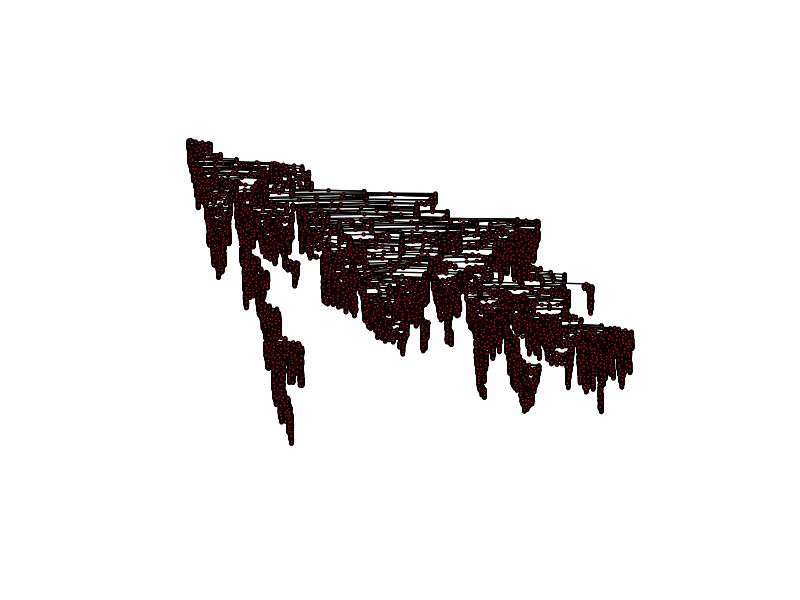
\includegraphics[width=10cm,height=6cm]{renduNX}
\end{center}
\end{figure}
	
	\section{Sans labels}
	
\paragraph{GraphViz}

\begin{figure}[h]
\begin{center}
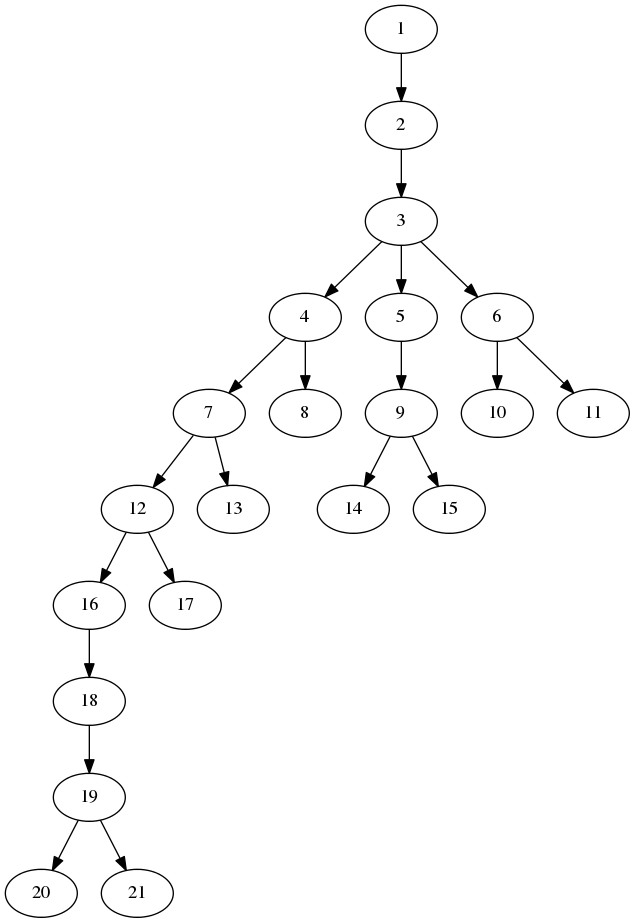
\includegraphics[width=0.75\columnwidth]{renduGVLabels}
\end{center}
\end{figure}

\paragraph{TikZ}

\begin{figure}[h] \centering \resizebox {!}{0.75\columnwidth} {
\begin{tikzpicture}[scale=0.8, every node/.style={scale=0.8}, node distance=1pt]
\node (a3027826572) at (3.500000, -0.000000) {1};
\node (a3027828524) at (3.500000, -1.000000) {2};
\node (a3027828204) at (3.500000, -2.000000) {3};
\node (a3027827948) at (2.000000, -3.000000) {4};
\node (a3027826636) at (1.500000, -4.000000) {7};
\node (a3027826988) at (1.000000, -5.000000) {12};
\node (a3027826604) at (0.500000, -6.000000) {16};
\node (a3027830572) at (0.500000, -7.000000) {18};
\node (a3027830092) at (0.500000, -8.000000) {19};
\node (a3027832332) at (0.000000, -9.000000) {20};
\draw (a3027830092) -- (a3027832332);
\node (a3027832396) at (1.000000, -9.000000) {21};
\draw (a3027830092) -- (a3027832396);
\draw (a3027830572) -- (a3027830092);
\draw (a3027826604) -- (a3027830572);
\draw (a3027826988) -- (a3027826604);
\node (a3027832556) at (1.500000, -6.000000) {17};
\draw (a3027826988) -- (a3027832556);
\draw (a3027826636) -- (a3027826988);
\node (a3027832684) at (2.000000, -5.000000) {13};
\draw (a3027826636) -- (a3027832684);
\draw (a3027827948) -- (a3027826636);
\node (a3027832812) at (2.500000, -4.000000) {8};
\draw (a3027827948) -- (a3027832812);
\draw (a3027828204) -- (a3027827948);
\node (a3027849356) at (3.500000, -3.000000) {5};
\node (a3027849388) at (3.500000, -4.000000) {9};
\node (a3027849420) at (3.000000, -5.000000) {14};
\draw (a3027849388) -- (a3027849420);
\node (a3027849516) at (4.000000, -5.000000) {15};
\draw (a3027849388) -- (a3027849516);
\draw (a3027849356) -- (a3027849388);
\draw (a3027828204) -- (a3027849356);
\node (a3027849676) at (5.000000, -3.000000) {6};
\node (a3027849708) at (4.500000, -4.000000) {10};
\draw (a3027849676) -- (a3027849708);
\node (a3027849804) at (5.500000, -4.000000) {11};
\draw (a3027849676) -- (a3027849804);
\draw (a3027828204) -- (a3027849676);
\draw (a3027828524) -- (a3027828204);
\draw (a3027826572) -- (a3027828524);

\end{tikzpicture}}
\end{figure}

\paragraph{Asymptote}

\begin{figure}[h]
\begin{asy}
size(20cm, 20cm);
label("1", (3.500000, -0.000000), E);
label("2", (3.500000, -1.000000), E);
label("3", (3.500000, -2.000000), E);
label("4", (2.000000, -3.000000), E);
label("7", (1.500000, -4.000000), E);
label("12", (1.000000, -5.000000), E);
label("16", (0.500000, -6.000000), E);
label("18", (0.500000, -7.000000), E);
label("19", (0.500000, -8.000000), E);
label("20", (0.000000, -9.000000), E);
draw((0.500000, -8.000000) -- (0.000000, -9.000000));
label("21", (1.000000, -9.000000), E);
draw((0.500000, -8.000000) -- (1.000000, -9.000000));
draw((0.500000, -7.000000) -- (0.500000, -8.000000));
draw((0.500000, -6.000000) -- (0.500000, -7.000000));
draw((1.000000, -5.000000) -- (0.500000, -6.000000));
label("17", (1.500000, -6.000000), E);
draw((1.000000, -5.000000) -- (1.500000, -6.000000));
draw((1.500000, -4.000000) -- (1.000000, -5.000000));
label("13", (2.000000, -5.000000), E);
draw((1.500000, -4.000000) -- (2.000000, -5.000000));
draw((2.000000, -3.000000) -- (1.500000, -4.000000));
label("8", (2.500000, -4.000000), E);
draw((2.000000, -3.000000) -- (2.500000, -4.000000));
draw((3.500000, -2.000000) -- (2.000000, -3.000000));
label("5", (3.500000, -3.000000), E);
label("9", (3.500000, -4.000000), E);
label("14", (3.000000, -5.000000), E);
draw((3.500000, -4.000000) -- (3.000000, -5.000000));
label("15", (4.000000, -5.000000), E);
draw((3.500000, -4.000000) -- (4.000000, -5.000000));
draw((3.500000, -3.000000) -- (3.500000, -4.000000));
draw((3.500000, -2.000000) -- (3.500000, -3.000000));
label("6", (5.000000, -3.000000), E);
label("10", (4.500000, -4.000000), E);
draw((5.000000, -3.000000) -- (4.500000, -4.000000));
label("11", (5.500000, -4.000000), E);
draw((5.000000, -3.000000) -- (5.500000, -4.000000));
draw((3.500000, -2.000000) -- (5.000000, -3.000000));
draw((3.500000, -1.000000) -- (3.500000, -2.000000));
draw((3.500000, -0.000000) -- (3.500000, -1.000000));
\end{asy}

\end{figure}

\paragraph{NetworkX}

\begin{figure}[h]
\begin{center}
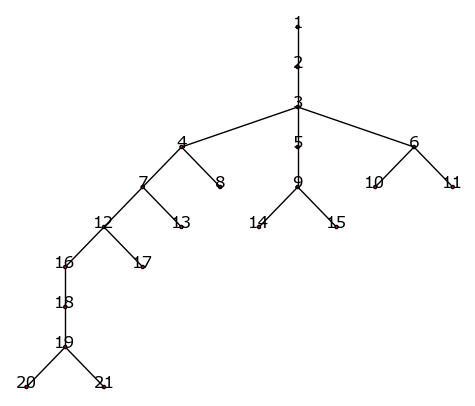
\includegraphics[width=0.75\columnwidth]{renduNXLabels}
\end{center}
\end{figure}